%  $Description: Thesis
%  $Author: xxx $
%  $Date: xxx  $
%  $Revision: 0.0 $

\documentclass[11pt]{book}
% \usepackage{iiit_thesis}
\usepackage{iiit_thesis_new}
% \usepackage{times}
\usepackage{epsfig}
% \usepackage{amsmath}
% \usepackage{amssymb}
% \usepackage{latexsym}
\usepackage{graphicx}
% \usepackage{multirow}
% \usepackage{algorithm2e}
\usepackage{listing}
\usepackage{times}
\usepackage{latexsym}
\usepackage{physics}
\usepackage{amsmath}
\usepackage{amssymb}
\usepackage{stmaryrd}
% \usepackage{tikz}
\usepackage{multirow}
\usepackage{multicol}
\usepackage{array}
\usepackage{amsthm}
\usepackage{mathtools}
\usepackage{booktabs}
\usepackage{epigraph}
\usepackage{todonotes}
% \usepackage{natbib}
% \bibliographystyle{unsrtnat}

% \usepackage{float} % use for H with figures, which forces figure locations.

\usepackage{tikz}
\usetikzlibrary{arrows}
\usetikzlibrary{shapes}
\newcommand*\circled[1]{\tikz[baseline=(char.base)]{
            \node[shape=circle,fill=pairedOneLightBlue,inner sep=1pt] (char) {#1};}}

\usepackage[sc,osf]{mathpazo}   % With old-style figures and real smallcaps.
\linespread{1.025}              % Palatino leads a little more leading
% Euler for math and numbers
\usepackage[euler-digits,small]{eulervm}

\usepackage[T1]{fontenc}
\usepackage{inconsolata}
\usepackage{lettrine}
\usepackage{yfonts}

\usepackage{amsmath}
\usepackage{amssymb}
\usepackage{amsthm}
\usepackage{minted}

\usepackage{hyperref}
\usepackage{cancel}
% \usepackage{mathtools}

% hyperlink colors
% https://tex.stackexchange.com/questions/823/remove-ugly-borders-around-clickable-cross-references-and-hyperlinks
\usepackage{xcolor}
\hypersetup{
    colorlinks,
    linkcolor={red!50!black},
    citecolor={red!50!black},
    urlcolor={red!50!black}
}


\newcommand{\skewsym}{\mathrm{Skew}}
\newcommand\ddfrac[2]{\frac{\displaystyle #1}{\displaystyle #2}}
\newcommand{\N}{\ensuremath{\mathbb{N}}}
\newcommand{\C}{\ensuremath{\mathbb{C}}}
\newcommand{\coT}{\ensuremath{T^*}}
\newcommand{\Lie}{\ensuremath{\mathfrak{L}}}
\newcommand{\Vectorfield}{\ensuremath{\mathfrak{X}}}
\newcommand{\pushforward}[1]{\ensuremath{{#1}_{\star}}}
\newcommand{\pullback}[1]{\ensuremath{{#1}^{\star}}}
\newcommand{\vectorfield}{\ensuremath{\mathfrak{X}}}
\newcommand{\Z}{\ensuremath{\mathbb Z}}
\newcommand{\pushfwd}[1]{\pushforward{#1}}
\newcommand{\pf}[1]{\pushfwd{#1}}

\newcommand{\boldX}{\ensuremath{\mathbf{X}}}
\newcommand{\boldY}{\ensuremath{\mathbf{Y}}}
%\renewcommand{\UrlFont}{\ttfamily\small}
\newcommand{\card}[1]{\left| #1 \right|}
\DeclarePairedDelimiterX{\infdivx}[2]{(}{)}{%
 #1\;\delimsize|\delimsize|\;#2%
}


\newcommand{\infdiv}{D\infdivx}

%\newcommand{\card}[1]{\ensuremath{\left| #1 \right|}}
\newcommand{\wtov}{\texttt{word2vec }}
\newcommand{\citep}[1]{\cite{#1}}
\newcommand{\citet}[1]{\cite{#1}}
\newcommand{\R}{\ensuremath{\mathbb R}}

\def\qed{$\Box$}
\newtheorem{theorem}{Theorem}
\newtheorem{corollary}[theorem]{Corollary}
\newtheorem{definition}[theorem]{Definition}
\newtheorem{lemma}[theorem]{Lemma}
\newtheorem{observation}[theorem]{Observation}
% \newtheorem{proof}[theorem]{Proof}
\newtheorem{remark}[theorem]{Remark}
\newtheorem{example}[theorem]{Example}

\definecolor{pairedNegOneLightGray}{HTML}{cacaca}
\definecolor{pairedNegTwoDarkGray}{HTML}{827b7b}
\definecolor{pairedOneLightBlue}{HTML}{a6cee3}
\definecolor{pairedTwoDarkBlue}{HTML}{1f78b4}
\definecolor{pairedThreeLightGreen}{HTML}{b2df8a}
\definecolor{pairedFourDarkGreen}{HTML}{33a02c}
\definecolor{pairedFiveLightRed}{HTML}{fb9a99}
\definecolor{pairedSixDarkRed}{HTML}{e31a1c}


\graphicspath{{figures/}{./}} % To include images in other directories

% https://tex.stackexchange.com/questions/132849/how-can-i-change-the-font-size-of-the-number-in-minted-environment
\renewcommand{\theFancyVerbLine}{\sffamily \textcolor[rgb]{0.2,0.2,0.2}{\small \oldstylenums{\arabic{FancyVerbLine}}}}


\long\def\symbolfootnote[#1]#2{\begingroup%
\def\thefootnote{\fnsymbol{footnote}}\footnote[#1]{#2}\endgroup}
\renewcommand{\baselinestretch}{1.2}
\onecolumn
%--------------------------------------------------------

\begin{document}
\pagenumbering{roman}

%% TITLE PAGE
\thispagestyle{empty}
\begin{center}
\vspace*{1.5cm}
{\Large \bf Mathematical Structures for Word Embeddings}

\vspace*{3.75cm}
{\large Thesis submitted in partial fulfillment\\}
{\large  of the requirements for the degree of \\}

\vspace*{1cm}
{\it {\large Master of Science in Computer Science and Engineering by Research} \\
% {\large in\\}
% {\large COURSE \\}}
}

\vspace*{1cm}
{\large by}

\vspace*{5mm}
{\large Siddharth Bhat\\}
{\large 20161105 \\
{\small \tt siddharth.bhat@research.iiit.ac.in }}


\vspace*{4.0cm}
{\psfig{figure=figures/iiit.eps,width=14mm}\\}
% {\large CSTAR: Center for Security, Theory, and Algorithms Research \\}
{\large International Institute of Information Technology\\}
{\large (Deemed to be University) \\}
{\large Hyderabad - 500 032, INDIA\\}
{\large November 2021 \\}
\end{center}


%% COPYRIGHT PAGE
\newpage
\thispagestyle{empty}
\renewcommand{\thesisdedication}{{\large Copyright \copyright~~Siddharth Bhat, 2021\\}{\large All Rights Reserved\\}}
\thesisdedicationpage

%% CERTIFICATE PAGE
\newpage
\thispagestyle{empty}
\vspace*{1.5cm}
\begin{center}
{\Large International Institute of Information Technology\\}
{\Large Hyderabad, India\\}
\vspace*{3cm}
{\Large \bf CERTIFICATE\\}
\vspace*{1cm}
\noindent
\end{center}
It is certified that the work contained in this thesis, titled `` '' by NAME, has been carried out under
my supervision and is not submitted elsewhere for a degree.

\vspace*{3cm}
\begin{tabular}{cc}
\underline{\makebox[1in]{}} & \hspace*{5cm} \underline{\makebox[2.5in]{}} \\
Date & \hspace*{5cm} Adviser: Prof. NAME
\end{tabular}
\oneandhalfspace

%%% DEDICATION PAGE
\newpage
\thispagestyle{empty}
\renewcommand{\thesisdedication}{\large To \texttt{\#math} \&\texttt{\#harmless}}
\thesisdedicationpage

\mastersthesis
\renewcommand{\baselinestretch}{1.5}

% ACKNOWLEDGEMENTS PAGE
\chapter*{Acknowledgments}
\label{ch:ack}
to \texttt{\#harmless} and \texttt{\#math}, for teaching me so much more than I
could possibly have learnt on my own; To \texttt{davean} for the uninvited
talk. To \texttt{topos} for all the category theory. To \texttt{ekmett} for
\texttt{\#harmless}. To \texttt{Z-module} to showing me the beauty of groups,
to \texttt{drazak} for teaching me orbit-stabilizer, to \texttt{dalcde} for
correcting my definition of compactness, to \texttt{antonfire} for yelling at
me when I didn't understand the totient, to \texttt{bgamari} for infinite
patience with dropped projects, to \texttt{PlanckWalk} for the patient
explanation of an elliptic PDE, to \texttt{Millennial} for a description of the
langlands, to \texttt{sure} for what a sheaf is, to all of you for making a
corner of the internet feel like home. To mona, for SpaG, britpick, coffee, and
tech support. To adlucem, for dubious frog chasing. To Superty, nitin, and our
goddess, for what is lost may be found again. ParticleMania and Itihas, thanks
for the many obtuse conversations that shaped what I thought. To Kannan and
Manish, and Venkatesh, for giving me the levity to pursue what I wanted. To
Uday, for the math, warmth, and opportunities. To Arnaud, for the many
conversations. To Tobias, for being a way better advisor than I  ever deserved.
To \texttt{Vyn} and \texttt{GodotMisogi}, for Math-Utopia. To \texttt{Luca},
\texttt{Senpai}, and \texttt{LLLB} for bake and pancakes. To
\texttt{codelegend}, for going along with my incorrect explanations. To panda,
for marx, coffee, and the baked potato recipe. To Goose, for all the physics.
To Ameya, Animesh, Aman,Athreya, Auro, Shaanjeet, and all the rest of theory
group for our shared love. To  Timo for mate, Tal for the coffee, Greg for the
cherry vodka. To all the folks at IISc, Tweag,  ETH, and theory group for the
great times. To Alok, for beginning this project in the first place. To mum,
for the cats and tea. To dad, for teaching me squeak.


%% ABSTRACT PAGE
\chapter*{Abstract}
\label{ch:abstract}
\epigraph{It is only proper to realize that language is largely a historical accident.}{John Von Neumann}

With the growing use of natural language processing tools (NLP) in
wide-ranging applications, it becomes imperative to understand why NLP models
are as successful as they are. In particular, it is essential to understand
what mathematical structures precisely underpin these models. To investigate
the mathematical models of NLP knowledge representations, we focus on the
setting of unsupervised word embeddings, due to the presence of robust models,
and a seemingly simple mathematical structure. We find that even in this
restricted setting, there are subtle, cross-cutting concerns as to how the
model learns --- beginning from the high level description of learning a
``vector'', to the low level details of implementations of these algorithms,
including initialization and gradient calculation. We build a theory of
knowledge representations for word embeddings, inspired by two seemingly
unrelated ideas (a) Montague semantics, a linguistic theory of meaning which
ascribes set-theoretic meaning to language, and (b) abstract interpretation, a
mathematical theory of creating computable approximations to uncomputable
semantics of programs. We find that syntheszing these ideas provide a way to
extract fuzzy-set embeddings from existing word-embeddings, which provides the
full range of set-theoretic operations (union, intersection, and others), along
with probabilistic operations (KL divergence, entropy) which are used to
perform polysemy detection and word sense disambiguation, while retaining
performance on regular word embeddings tasks such as similarity. Next, we turn
our attention to generalizing the word embedding training regime by extracting
the geometry which is currently held implicit. This leads us to formulate a
general theory of learning word representations on Lie groups. In summary, we
provide insight into the mathematical structure of word representations.



\tableofcontents
\listoffigures
\listoftables
%--------------------------------------------------------
\pagenumbering{arabic}

\chapter{Introduction}

\epigraph{The sky is the limit, so lets build rockets!}{Anonymous}


% \textinit{N}atural language processing has, since its inception, required
Natural language processing has, since its inception, required
techniques to extract semantic information from raw corpora with little to no
supervision. To perform such unsupervised learning, many models
have been built, based off of the ``Distributional Hypothesis'', which states
that words that occur in the same contexts tend to have similar meanings.
\todo{Harris 1954 is also a citation here}
The
underlying idea that ``a word is characterized by the company it keeps'' was
popularized by Firth \citep{firth1957synopsis}.

An early technique which exploited distributional semantics was Latent Semantic
Analysis (LSA) \cite{landauer1998introduction}. LSA analyzes relationships by
assuming that words that are close in meaning will occur in similar pieces of
text (the distributional hypothesis), and thus matrix containing word counts
per document (rows represent unique words and columns represent each document)
is constructed from a large piece of text and  singular value decomposition
(SVD) is used to reduce the number of rows while preserving the similarity
structure among columns. Documents are then compared by taking the cosine of
the angle between the two vectors, where angles close to $1$ represent very
similar documents, and angles close to $0$ represent dis-similar documents.

\texttt{Word2vec} is a recent technique to create unsupervised word embeddings
for NLP from unstructured data, whose informal correctness is based on the
distributional hypothesis. \todo{citations on both word2vec and correctness}
The \texttt{word2vec} algorithm uses a neural network \todo{neural network?}
model to learn word associations from a large corpus of text. Once trained,
such a model can detect synonymous words or suggest additional words for a
partial sentence.  As befitting the name, \texttt{word2vec} represents each
distinct word with a vector. \todo{Nitpick: it is every surface form which is a
  vector, because I would argue bank and bank are different words.}
The training mechanism yields vectors such that
the cosine of the angle between the vectors reflects the the level of semantic
similarity between the words represented by those vectors.

On the other hand, it is very unclear why the \texttt{word2vec} training regime
is as successful as it is. \todo{citation}
In comparison to LSA, which has theoretical guarantees
since it is based on linear-algebraic ideas such as SVD, the correctness of
\texttt{word2vec} is far less clear. In this thesis, we \todo{I've been told we
  write `I' in theses, as technically you're the only one writing it.}
attempt to provide a
\emph{linguistically} as well as \emph{mathematically} motivated explanation
for the correctness of \texttt{word2vec}. We begin with a deep dive into the \texttt{word2vec}
implementation. Following this, we chase a \emph{linguistic} theory of meaning,
by considering \emph{Montague semantics}. Developing on this idea, we borrow the tools of
\emph{Abstract Interpretation} \cite{cousout1996abstract}, a technique development in computer science for
program analysis, which is used to approximate the (formal) meaning/semantics
of a program. Using abstract interpretation, we propose a scheme to extract
\emph{Montagueian semantics} from \texttt{word2vec}, and evaluate the
performance of our proposed system. Finally, we generalize \texttt{word2vec}
far beyond its original setting. Concretely, we tackle the following questions:

\begin{enumerate}
    \item How \texttt{word2vec} \emph{really} works, including an
        investigation of all the tricks that are used in its reference C
        implementation and the bearings they have on the quality of the
        generated word vectors. This is answered in \autoref{chapter:deep-dive-wtov},
        where we analyze the \texttt{word2vec} sources and extract insights from this process.
    \item What is a general theory of meaning that can be adapted to
        statistical machine learning? Why is abstract interpretation a
        potential candidate? This is answered in \autoref{chapter:abstract-interpretation},
        where we explain Abstract Interpretation, and link this theory to Montague semantics.
    \item How can Abstract Interpretation be melded into the \texttt{word2vec}
        training regime? This is answered in
        \autoref{chapter:fuzzy-set-representation}, where we create new
        \emph{fuzzy embeddings} and evaluate their effectiveness.
    \item What is the largest setting where \texttt{word2vec} can be
        implemented? In particular, how much of the mathematical structure of a
        vector is exploited by \texttt{word2vec} embeddings, and by how much
        can we generalize this training regime? This is answered in
        \autoref{chapter:geometrization} where we generalize \texttt{word2vec} to arbitrary Lie groups.
\end{enumerate}



\chapter{Background}
\section{A deep dive into \wtov}
\label{chapter:deep-dive-wtov}

\epigraph{He turned back to face them. ‘I do make sense to you, don’t I? I’m not just imagining that communication is taking place?'}{Greg Egan}

% \textinit{T}he popular opinion in the NLP literature
The popular opinion in the NLP literature
is that that systems such as \texttt{word2vec} learn
vector representations \cite{levy2014neural}, \cite{pennington2014glove}.  A word
embedding learned as a vector, where words with a similar meaning can be given
similar vectors. More specifically, the aim of providing vector representations
to words is to understand that words that occur in \textit{similar contexts}
should be given ``similar'' vectors. While \wtov was not the first mechanism to
think of embedding words in a vector space
\cite{baroni2010distributional,bruni2012distributional}. However, it is the
first which achieved an efficient regime for training and the requisite
reduction in dimensionality for storing and evalution, thereby making it a
benchmark for modern natural language processing. However, few in-depth analyses
of the model and \textit{why} it is accurate in downstream tasks and efficient
to train made it an important development in the field.


Hence, this forms as the launching point for our study. We will
first describe the popular description of the algorithm as found online, describe
gaps in both the online descriptions and in the original paper. Next, we dissect the
source code of \texttt{word2vec}. Armed with detailed knowledge of the real
training mechanism, we lay out the list of open questions in the design of
\texttt{word2vec}. \todo{talk about evaluation, not just training, because fuzzy
  had insight into asymmetric eval metrics as well}
To answer these questions, we explain the mathematical
theory of abstract interpretation and connect this to montague semantics in
\autoref{chapter:abstract-interpretation}, and we then use this to build fuzzy
set representations in \autoref{chapter:fuzzy-set-representation}.

\subsection{\wtov in the literature}

\begin{figure}[htb]
\begin{minted}[linenos]{cpp}
Maintain a word -> vector mapping.
while(1) {
  vf = vector corresponding to focus word
  vc = vector corresponding to context word
  train such that (vc . vf = 1)
  for(0 <= i < negative samples):
  vneg = vector of word *not* in context
  train such that (vf . vneg = 0)
}
\end{minted}
\caption{word2vec:  high-level \emph{incorrect} pseudocode. This is the popular
    explanation of available on Wikipedia and the TensorFlow page.}
\label{fig:wrong-w2v-pseudocode}
\end{figure}

% TODO: fix the wikipedia implementation
% Indeed, if I google "word2vec skipgram", the results I get are:
% - [The wikipedia page which describes the algorithm on a high level](https://en.wikipedia.org/wiki/Word2vec#Training_algorithm)
% - [The tensorflow page with the same explanation](https://www.tensorflow.org/tutorials/representation/word2vec)
% - [The towards data science blog which describes the same algorithm](https://towardsdatascience.com/word2vec-skip-gram-model-part-1-intuition-78614e4d6e0b)
%
% The list goes on. However, __every single one of these implementations is wrong__.

The classic explanation of \texttt{word2vec}, in skip-gram, with negative
sampling is the pseudocode shown in \autoref{fig:wrong-w2v-pseudocode}. The paper
is arguably too terse to extract out any pseudocode from, so we thus defer to the
explanations available on \href{https://en.wikipedia.org/wiki/Word2vec#Training_algorithm}{Wikipedia}
and the \href{https://www.tensorflow.org/tutorials/representation/word2vec}{TensorFlow} re-implementation.

The original \wtov \texttt{C} implementation does not do what is explained above.
serious users of word embeddings either (a) directly invoke the original C
implementation of \texttt{word2vec}, or (b) invoke the \texttt{gensim}
implementation \cite{vrehuuvrek2011gensim}, which is \emph{transliterated} from the C source to the extent
that the variables names are the same as that of the C implementation.
\todo{gensim implementation links}
Hence, we shall read the source code to
better understand the training scheme of \texttt{word2vec}.

\subsection{\wtov in the sources}

We analyze the original C implementation of \texttt{word2vec}, to point out
salient features, curious implementation decisions and bugs in the
implementation \todo{why not the master branch directly?}
\footnote{sources taken from \url{https://github.com/tmikolov/word2vec/blob/20c129af10659f7c50e86e3be406df663beff438/word2vec.c}}.
This necessitates interleaving high level explanations with direct snippets of  C source code;
We do not apologize for this. We view this as a feature of this thesis, not a bug, since we deal
with details such as the initialization and gradient calculations.  The core
training loop of \wtov (trained using negative sampling, in skip-gram mode)
ingests a corpus, and then attempts to learn \emph{two} representations for a
given word, called as the positive and negative representation. At a high
level, the python pseudocode at \autoref{fig:w2v-py-pseudocode} explains the
implementation of \texttt{word2vec}.


\subsubsection{Initialization}
(a) An array called `syn0` holds the vector embedding of a word when it occurs
as a \emph{focus word}. This is random initialized.

\begin{minted}{cpp}
// tmikolov/word2vec/blob/20c129af10659f7c50e86e3be406df663beff438/word2vec.c#L369
for (a = 0; a < vocab_size; a++) for (b = 0; b < layer1_size; b++) {
 next_random = next_random * (unsigned long long)25214903917 + 11;
 syn0[a * layer1_size + b] =
 (((next_random & 0xFFFF) / (real)65536) - 0.5) / layer1_size;
}
\end{minted}

(b) Another array called \texttt{syn1neg} holds the vector of a word when it occurs
as a \emph{context word}. This is zero initialized.

\begin{minted}{cpp}
// tmikolov/word2vec/blob/20c129af10659f7c50e86e3be406df663beff438/word2vec.c#L365
for (a = 0; a < vocab_size; a++) for (b = 0; b < layer1_size; b++)
syn1neg[a * layer1_size + b] = 0;
\end{minted}


\subsubsection{Training}

During training (skip-gram, negative sampling, though other cases are
also similar), we first pick a focus word. This is held constant throughout
the positive and negative sample training. The gradients of the focus vector
are accumulated in a buffer, and are applied to the focus word
\emph{after} it has been affected by both positive and negative samples.
Line number \circled{4} decides whether we are picking a positive sample (\texttt{d = 0})
or a negative sample (\texttt{d > 0}). If we are picking a positive sample, then we expect
at \circled{5} to find the dot-product with the \texttt{word} to be \texttt{1}.
On the other hand, if we are picking a negative sample, then we expect at \circled{10} to pick
a random word, and at \circled{13} for the dot-product to be zero. \circled{20} computes
the dot-product between the focus word and the picked context word.
\circled{23}-\circled{25} computes the gradient $g \equiv \sigma(\texttt{label} - \texttt{focus} \cdot \texttt{ctx})$.
\circled{30}-\circled{31} performs the backprop of the loss of the focus and context word. Note that
the gradient of the focus word is stored into a buffer \texttt{neu1e}. This ensures that the gradient of
the focus word is held constant throught the positive and negative samples. Finally, on
\circled{36}, the buffered gradient \texttt{neu1e} is propagated into the focus word.


\begin{minted}[linenos]{cpp}
for (d = 0; d < negative + 1; d++) {
 // if we are performing negative sampling, in the 1st iteration,
 // pick a word from the context and set the dot product target to 1
 if (d == 0) {
   target = word; label = 1;
 } else {
   // for all other iterations, pick a word randomly and set the dot
   //product target to 0
   next_random = next_random * (unsigned long long)25214903917 + 11;
   target = table[(next_random >> 16) % table_size];
   if (target == 0) target = next_random % (vocab_size - 1) + 1;
   if (target == word) continue;
   label = 0;
 }
 l2 = target * layer1_size;
 f = 0;

 // find dot product of original vector with negative sample vector
 // store in f
 for (c = 0; c < layer1_size; c++) f += syn0[c + l1] * syn1neg[c + l2];

 // set g = sigmoid(f) (roughly, the actual formula is slightly more complex)
 if (f > MAX_EXP) g = (label - 1) * alpha;
 else if (f < -MAX_EXP) g = (label - 0) * alpha;
 else g = (label - expTable[(int)((f + MAX_EXP) * (EXP_TABLE_SIZE / MAX_EXP / 2))]) * alpha;

 // 1. update the vector syn1neg,
 // 2. DO NOT UPDATE syn0
 // 3. STORE THE syn0 gradient in a temporary buffer neu1e
 for (c = 0; c < layer1_size; c++) neu1e[c] += g * syn1neg[c + l2];
 for (c = 0; c < layer1_size; c++) syn1neg[c + l2] += g * syn0[c + l1];
}
// Finally, after all samples, update syn1 from neu1e
// tmikolov/word2vec/blob/20c129af10659f7c50e86e3be406df663beff438/word2vec.c#L541
// Learn weights input -> hidden
for (c = 0; c < layer1_size; c++) syn0[c + l1] += neu1e[c];
\end{minted}



\subsubsection{Summary}

We outline what we have learnt from delving into the C sources
of \wtov to provide high-level pseudocode of the algorithm.

\begin{figure}[htb]
\begin{minted}{python}
def learn(lix: int, rix:int, larr:np.array, rarr:np,array,
  out :float, target: float):
  # gradient descent on loss (target - out)^2 where
  gloss = 2 * (target - out)
  pass

def train(corpus):
  poss = np.array((VOCABSIZE, DIMSIZE))
  negs = np.array((VOCABSIZE, DIMSIZE))

  for wix in range(len(corpus)):
    w = poss[corpus[wix]]
    l = max(wix-WINDOWSIZE, 0)
    r = min(wix+WINDOWSIZE, len(corpus)-1)

    for xix in range(l, r+1):
        x = poss[xix]
        out = np.dot(x, w)
        learn(lix=wix, rix=xix, larr=poss, rarr=poss, out=out, target=1.0)

    for _ in range(NNEGSAMPLES)
        xix = random.randint(0, len(corpus)-1)
        x = negs[xix]
        out = np.dot(x, w)
        learn(lix=wix, rix=xix, larr=poss, rarr=negs, out=out, target=0.0)
\end{minted}
\caption{\texttt{word2vec} pseudocode, explaining the core training algorithm}.
\label{fig:w2v-py-pseudocode}
\end{figure}

\subsection{Bugs}

In this subsection, we list bugs that were discovered by us in the \texttt{word2vec}
codebase. While these do not impact training significantly, they do point out
the dangers of using C as programming language, as well as provides justification
for reading the original sources.

\subsubsection{Epoch resetting}

\begin{minted}[linenos]{cpp}
if (eof || (word_count > train_words / num_threads)) {
  word_count_actual += word_count - last_word_count; local_iter--;
  if (local_iter == 0) break;
  word_count = 0; last_word_count = 0; sentence_length = 0;
  // eof = 0; /* Missing code! */
  fseek(fi, file_size / (long long)num_threads * (long long)id,
     SEEK_SET);
  continue;
}
\end{minted}

\texttt{word2vec} trains on multiple threads in parallel. The thread that reads
the final chunk of text does not reset its \texttt{eof} (end-of-file) state
upon reaching the end of file. The code at line \circled{5} ought to have been present,
but is missing. Thus, the final fragment of text is trained for only a single
epoch, which causes the word vectors to miss data about the last section of the document.
This causes the overall accuracy  to be lowered than the potential optima.

\subsubsection{Initialization choices}

We conjecture that since the negative samples come from all over the text and
are not really weighed by frequency, you can wind up picking \emph{any word},
and more often than not, \emph{a word whose vector has not been trained much at
all}.  If this vector actually had a value, then it could move the actually
important focus word randomly. The solution is to set all negative samples to
zero, so that \emph{only vectors that have occurred somewhat frequently} will
affect the representation of another vector. This also explains GloVe's radical
choice of having a separate vector for the negative context --- they re-used
\wtov's  scheme, re-interpreting the negative vector and positive vector as
accounting for different aspects of co-occurence.

\todo{Nothing on the threading issues? The fact that changing the number of
  threads actually either crashed the training or didn't train a certain
  arbitrary group of words iirc?}

\subsubsection{Relationship to GloVe}

The \texttt{C} implementation in fact maintains \emph{two vectors for each word}, one where
it appears as a focus word, and one where it appears as a context word.
(Is this sounding familiar? Indeed, it appears that GloVe actually took this
idea from `word2vec`, which has never mentioned this fact!) \todo{MAKE MORE FORMAL,
  citation, code link in footnotes}


\subsubsection{Conclusions on \texttt{word2vec}}

The output of the training regime are popularly interpreted as vectors.
However, we augment this discussion by bringing in nuance. In particular, we
note that:
\begin{itemize}
\item Scalar multiples of the same vector represent the same concept as per the testing regime.
\item Vector addition has no clear meaning in the representation.
\item The identity element (the zero vector) holds no semantic meaning in the representation.
\item The reality of the training regime as-implemented makes it unclear as to
      what mathematical object is being learnt.
\end{itemize}


We learn that the \texttt{word2vec} training regime creates two sets of vectors, henceforth
referred to as \texttt{syn0} and \texttt{syn1neg}. The negative vectors
\texttt{syn1neg} are thrown away, while the positive vectors \texttt{syn0} are
the ones that are left at the end. The training regime \emph{does not use}
gradient descent. Rather, a style of perceptron-based \textit{batch} update is used.

Thus,
this leaves the question open as to what is really being learnt by
\texttt{word2vec}. We answer this question by hypothesizing that the
representation that is learnt by \texttt{word2vec} in fact encodes \emph{sets
of word senses}, which we extract from \texttt{word2vec} by using ideas of
abstract interpretation. We explain the ideas of abstract interpretation in
\autoref{chapter:abstract-interpretation}, and then proceed to use these ideas
to build fuzzy set representations in
\autoref{chapter:abstract-interpretation}. Finally, we propose an abstract
version of the \texttt{word2vec} training algorithm on any choice of Lie group
in \autoref{chapter:geometrization}.

\section{Abstract Interpretation}
\label{chapter:abstract-interpretation}
\epigraph{Among the thousand-and-one faces whereby form chooses to reveal itself to us, the one that fascinates me more than any other, and continues to fascinate me, is the structure hidden in mathematical things.}{Alexander Grothendieck}

% \textinit{A}bstract interpretation is a mathematical theory of approximation of meaning.
Abstract interpretation is a mathematical theory of approximation of meaning.
It was created by Cousout and Cousout to unify many disparate program analysis
techniques, such as dataflow analysis \emph{khedker2017data} and type checking
\cite{file199abstract}. The broad idea is to approximate the uncomputable,
real semantics of a program into an approximate, computable semantics.
The loss of information suffered during te process of abstraction is the price
one pays to allow the abstract domain be \emph{computable}, thereby providing
the ability to approximate concrete meaning. 

In the most general setting, an abstract interpretation is a manifestation of
an \emph{adjunction}, a mathematical structure which captures a notion of
"approximate inverses". It will be too much of a detour to explore the vast
land of categories and adjunctions. Suffice to say that many of the deep ideas
of mathematics arise out of adjunctions. Here, we shall focus on the special
case of an adjunction for lattices, known as a \emph{Galois connection}
\cite{cousout1992comparing}. We will show how the notion of a Galois connection
provides a good notion of "approximation of meaning", and how this directly
relates to Montague's ideas of representing semantics as subsets.

\subsection{Abstracting away even-ness}

Consider a notion of "odd" and even", and how we can generalize this notion to
arbitrary subsets of the integers.  Let us consider two lattices, $L \equiv
2^\Z$, the set of subsets of the integers, and $L^\sharp \equiv \{\bot, O, E,
\top\}$, the odd-even lattice. We define two functions, the abstract function
$\alpha: L \rightarrow L^\sharp$ which abstracts away information about subsets
of the integers into \texttt{even} and \texttt{odd}, and the concretization
function $\gamma: L^\sharp \rightarrow L$ which concretizes the idea of
even-ness and odd-ness into subsets of the integers. The abstraction function
maps the empty subset to $\bot$, since we know nothing about an empty set. It
maps sets of integers that are all even to $E$, since such a set is "even".
Similarly, it maps set of integers that are all odd to  $O$, since such a set
is "odd". For sets that contain a mixture of both even and odd, it maps these
top $\top$ to indicate "failure".

\[
	\alpha: 2^\Z\rightarrow L^\sharp; \quad
	\alpha(S) \equiv
	\begin{cases}
		\bot & S = \emptyset \\
		E & \text{$S$ contains only even numbers} \\
		O & \text{$S$ contains only odd numbers} \\
		\top & \text{otherwise}
	\end{cases}
\]

The concretization function attempts to make the idea of \emph{even} and
\emph{odd} concrete, by sending the concepts $\bot, E, O, \top$ to the sets
that best represent them. This is given by:

\begin{align*}
&\gamma: L^\sharp \rightarrow 2^\Z \\
&\gamma(\bot) \equiv \emptyset; \quad \gamma(\top) \equiv \Z; \\
&\gamma(E) \equiv \{ 2 k : k \in \in \Z\}; \quad
\gamma(O) \equiv \{ 2k + 1: k \in \Z \}
\end{align*}

That is, $\gamma$ maps $E$ to the even numbers, $O$ to the set of all odd
numbers, $\bot$ to the empty set, and $\top$ to the set of all numbers, since
we know nothing. Let's explore the relationship between $\alpha$ and $\gamma$.
What happens  when we consider the compositions $\alpha \circ \gamma$ (read as
"$\alpha$ after $\gamma$") and $\gamma \circ alpha$?

\begin{figure}[htb]
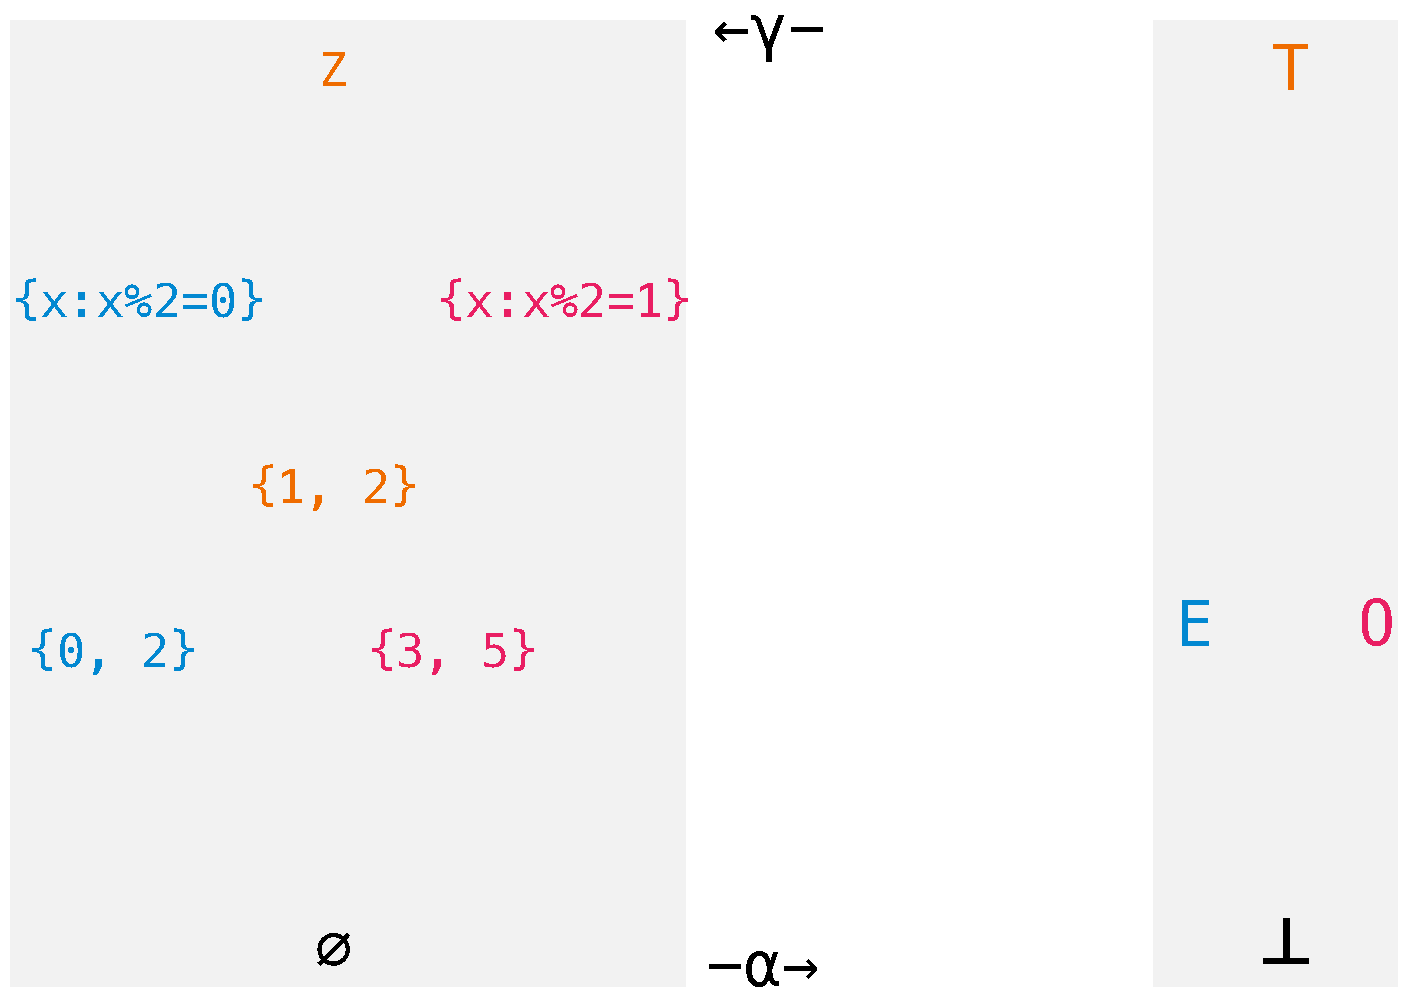
\includegraphics[width=\textwidth]{./abstract-interpretation.pdf}
\caption{Abstract interpretation of the Odd/Even lattice.}
\end{figure}

This leads us to the following relations:

\begin{align*}
	&C \subseteq (\gamma\circ \alpha)(C) \\
	&a = (\alpha \circ \gamma)(a) \\
\end{align*}

These first equation tell us that abstracting a concrete idea $C$ into
$\alpha(C)$ and then concretizing the abstract idea using $\gamma(\alpha(C))$
creates a loss of information. This captures the intuition that the abstraction
is lossy. The second equation tells us that if we start with an abstract object
$a$, then concretize it with $\gamma(a)$, this loses no information; Bringing
it back up to the abstract world with $alpha(\gamma(a)))$ recovers the $a$.
\subsubsection{Interval domain}


A second example is that of the interval domain, where we map subsets of the
integers $2^\Z$ to \emph{intervals} of the integers. The interval domain is a
less trivial domain that showcases conjunction and disjunction. For this
purpose, we pursue this example as well.  Our abstract domain $I \equiv Z
\times Z$ represents closed intervals. So an element $(1, 3) \in I$ is an
abstract representation of the closed interval $[1, 3] = \{ 1, 2, 3 \}$.  Similarly,
the element $(1, 0) \in I$ is an abstract representation of the interval $[1, 0] = \emptyset$,
as there is no interval whose leftmost point is $1$ and rightmost point is $0$.
In this case, the abstraction function $\alpha: L \rightarrow L^\sharp$ goes
from a set of integers to the smallest interval containing these numbers. For
example, $\alpha(\{1, 2, 3\}) = (1, 3)$, and $\alpha(\{1, 5\}) = (1, 3, 5)$.
See that the latter is an approximation: we are representing the triple of
numbers $1, 3$ and $5$ by the \emph{whole interval} $(1, 5)$, which we think of
as $\{1, 2, 3, 4, 5\}$. To make this formal, we define the concretization
function $\gamma: L^\sharp \rightarrow L$, where $\gamma((l, r)) \equiv \{ x
\in \mathbb Z : l \leq x \leq r \}$.


To define \emph{union} and \emph{intersection} of our intervals, we intuitively
want toe \emph{union} of two intervals to be the smallest interval that \emph{contains} them.
Similarly, we want the \emph{intersection} of two intervals to be the \emph{largest} interval
\emph{contained} in both of them. These are given by the definitions:

% https://scicomp.stackexchange.com/a/26260/31940
\begin{align*}
    &\sqcap^\sharp: L^\sharp \times L^\sharp \rightarrow L \quad (l, r) \sqcap (l', r') \equiv
    \begin{cases}
        (1, 0) & r < l' \lor r' < l \\
        (\max (l, l'), \max (r, r')) & \text{otherwise}
    \end{cases} \\
    &\sqcup^\sharp: L^\sharp \times L^\sharp \rightarrow L \quad (l, r) \sqcup (l', r') \equiv (\min(l, l'), \max(r, r'))
\end{align*}

Given two subsets $S, T \subseteq 2^\Z$, $\alpha(S \cap T)$ is the largest interval
containing elements of both $S$ and $T$. $\alpha(S) \sqcap^\sharp \alpha(T)$ is the
intersection of intervals containing $S$ and $T$, which is also the largest interval
containing both $S$ and $T$. Similarly, for union, we have the equation
$\alpha(S \cup T) = \alpha(S) \sqcup^\sharp \alpha(T)$

This shows that the theory of abstract interpretation is compatible with set
operations. In particular, the theory of abstract interpretation is capable of
abstracting notions of union and intersection, since the union and intersection
of the sets of integers is approximated by joins and meets in the abstract even-odd
lattice.


\subsection{The formal viewpoint}

A partial order is a set $L$ equipped with a binary relation $\leq \subseteq L
\times L$ which is (a) reflexive ($a \leq a$), (b) anti-symmetric $a \leq b
\land b \leq a \implies a = b$, and (c) transitive: $a \leq b \land b \leq c
\implies a \leq c$.  A monotone map is a morphism of partial orders. Formally,
it is a function $f: (L, \leq) \rightarrow (L^\sharp, \leq^\sharp)$ such that
$a \leq b \implies f(a) \leq^\sharp f(b)$.  A galois connectio between two
lattice $(L, \leq)$ and $(L^\sharp, \leq^\sharp)$ is a pair of monotone maps
$F: (L, \leq) \rightarrow (L^\sharp, \leq^\sharp)$, and
$G: (L^\sharp, \leq^\sharp) \rightarrow  (L, \leq)$ such that:

$$
a \leq F(b) \iff a \leq G(b)
$$

This is equivalent to the pair of conditions:

$$
a \leq F(G(a)); \quad b \leq G(f(b))
$$


\subsection{Montague semantics}

Montague grammar is an approach to natural language semantics pioneered by
Richard Montague. \todo{citation} The Montague grammar is based on mathematical logic.
Montague held the view that natural language was a formal language very much in
the same sense as predicate logic was a formal language. As such, in Montague’s
view, the study of natural language belonged to mathematics. To quote:

\begin{quote}
There is in my opinion no important theoretical difference between natural
languages and the artificial languages of logicians; indeed I consider it
possible to comprehend the syntax and semantics of both kinds of languages
with a single natural and mathematically precise theory.
\end{quote}

Montague semantics is used to describe the semantic properties of language.
Broadly speaking, a sentence is given meaning by constructing the set of all
possible worlds where that sentence is true. For a mathematical example, the
sentence $l \equiv (\forall x \in \Z, x < 2)$ is given meaning by constructing
the set $S_l \equiv \{ x \in \Z : x < 2 \} = \{1, 0, -1, \dots \}$. A false
proposition, such that $l' \equiv \forall x \in \Z, x > x + 1$ is given meaning
by the \emph{empty set} $S_{l'} \equiv \{ x \in \Z: x > x + 1 \} = \emptyset$.
As a linguistic example, the meaning of walk, or sing is defined as the set of
individuals who share respectively the property of walking or the property of
singining.  By appealing to the principle of compositionality, if there is a
rule that combines these two expressions to the verb phrase walk and sing,
there must be a corresponding rule that determines the meaning of that verb
phrase. In this case, the resulting meaning will be the \emph{intersection} of
the two sets.  Thus, the meaning of walk and sing is a subset of the meaning of
walk.

Ambiguity is dealt with by constructing sets which capture \emph{all possible
meanings}.  For example, the sentence ``Every man loves a woman'' can be ascribed
multiple meanings: (a) Every man loves the \emph{same} woman (say, Lilith), or
(b) every man loves a \emph{different} woman. This is dealt with by considering
the union of \emph{both sets of meanings}. To resolve ambiguity given more
context, we intersect the union of both sets of meaning with the correct context.

We see that compositionality arises naturally from set-theoretic semantics; it
is one of the cruxes of Montague's ``theory of meaning'', which was expanded
upon by the denotational semantics school of thought, where syntax and
semantics are algebra, and denotation, or meaning, is a morphism between them.
In our work, we exploit Montague semantics as the bridge to connect \texttt{word2vec} with
\todo{In my work, I ... <all the way through>}
abstract interpretation and fuzzy sets. We conjecture that \texttt{word2vec}
computes a sequence of abstract interpretations, first from the uncomputable
semantics of natural language that of the uncomputable montagueian semantics.
We conjecture that systems such as \texttt{word2vec} themselves compute another
layer of abstract interpretation. We attempt to extract evidence for this, and
come up non-empty-handed.


\chapter{Fuzzy set representations}
\label{chapter:fuzzy-set-representation}

\epigraph{And if we tamper with our inheritance, so what? What is more ours to tamper with?}{Ian M Banks}

% \textinit{W}e provide an alternate perspective on word representations, by
We provide an alternate perspective on word representations, by
reinterpreting the dimensions of the vector space of a word embedding as a
collection of features. In this reinterpretation, every component of the word
vector is normalized against all the word vectors in the vocabulary. This idea
now allows us to view each vector as an $n$-tuple (akin to a fuzzy set), where
$n$ is the dimensionality of the word representation and each element
represents the probability of the word possessing a feature. Indeed, this
representation enables the use fuzzy set theoretic operations, such as union,
intersection and difference. Unlike previous attempts, we show that this
representation of words provides a notion of similarity which is inherently
asymmetric and hence closer to human similarity judgements. We compare the
performance of this representation with various benchmarks, and explore some of
the unique properties including function word detection, detection of
polysemous words, and some insight into the interpretability provided by set
theoretic operations.

\section{Introduction} \label{sec: intro}

Word embedding is one of the most crucial facets of Natural Language Processing
(NLP) research. Most non-contextualized word representations aim to provide a
distributional view of lexical semantics, known popularly by the adage
\textit{"a word is known by the company it keeps"} \citep{firth1957synopsis}.
Popular implementations of word embeddings such as word2vec
\citep{mikolov2013efficient} and GloVe \citep{pennington2014glove} aim to
represent words as embeddings in a vector space. These embeddings are trained
to be oriented such that vectors with higher similarities have higher dot
products when normalized. Some of the most common methods of intrinsic
evaluation of word embeddings include similarity, analogy and compositionality.
While similarity is computed using the notion of dot product, analogy and
compositionality use vector addition.
\todo{not needed, already used in introduction}
However, distributional representations of words over vector spaces have an
inherent lack of interpretablity \citep{goldberg2014word2vec}. Furthermore, due
to the symmetric nature of the vector space operations for similarity and
analogy, which are far from human similarity judgements
\citep{tversky1977features}. Other word representations tried to provide
asymmetric notions of similarity in a non-contextualized setting, including
Gaussian embeddings \citep{vilnis2014word} and word similarity by dependency
\citep{gawron2014improving}. However, these models could not account for the
inherent compositionality of word embeddings \citep{mikolov2013distributed}.

Moreover, while work has been done on providing entailment for vector space
models by entirely reinterpreting word2vec as an entailment based semantic
model \citep{henderson2016vector}, it requires an external notion of
compositionality. Finally, word2vec and GloVe, as such, are meaning conflation
deficient, meaning that a single word with all its possible meanings is
represented by a single vector \citep{camacho2018word}. Sense representation
models in non-contextualized representations such as multi-sense skip gram, by
performing joint clustering for local word neighbourhood. However, these sense
representations are conditioned on non-disambiguated senses in the context and
require additional conditioning on the intended senses \citep{li2015multi}.

In this paper, we aim to answer the question: \textit{Can a single word
representation mechanism account for lexical similarity and analogy,
compositionality, lexical entailment \textbf{and} be used to detect and resolve
polysemy?} We find that by performing column-wise normalization of word vectors
trained using the word2vec skip-gram negative sampling regime, we can indeed
represent all the above characteristics in a single representation. We
interpret a column wise normalized word representation. We now treat these
representations as fuzzy sets and can therefore use fuzzy set theoretic
operations such as union, intersection, difference, etc. while also being able
to succinctly use asymmetric notions of similarity such as K-L divergence and
cross entropy. Finally, we show that this representation can highlight
syntactic features such as function words, use their properties to detect
polysemy, and resolve it qualitatively using the inherent compositionality of
this representation.

In order to make these experiments and their results observable in general, we
have provided the code which can be used to run these operations. The code can
be found at \url{https://github.com/AlokDebnath/fuzzy_embeddings}. The code
also has a working command line interface where users can perform qualitative
assessments on the set theoretic operations, similarity, analogy and
compositionality which are discussed in the paper.

\section{Related Work} \label{sec: related}

The representation of words using logical paradigms such as fuzzy logic,
tensorial representations and other probabilistic approaches have been
attempted before. In this section, we uncover some of these representations in
detail.

\citet{lee1999measures} introduced measures of distributional similarity to
improve the probability estimation for unseen occurrences. The measure of
similarity of distributional word clusters was based on multiple measures
including Euclidian distance, cosine distance, Jaccard's Coefficient, and
asymmetric measures like $\alpha$-skew divergence.

\citet{bergmair2011monte} used a fuzzy set theoretic view of features
associated with word representations. While these features were not adopted
from the vector space directly, it presents a unique perspective of entailment
chains for reasoning tasks. Their analysis of inference using fuzzy
representations provides interpretability in reasoning tasks.

\citet{grefenstette2013towards} presents a tenosrial calculus for word
embeddings, which is based on compositional operators \emph{which uses} vector
representation of words to create a compositional distributional model of
meaning. By providing a category-theoretic framework, the model creates an
inherently compositional structure based on distributional word
representations. However, they showed that in this framework, quantifiers could
not be expressed.

\citet{herbelot2015building} refers to a notion of general formal semantics
inferred from a distributional representation by creating relevant ontology
based on the existing distribution. This mapping is therefore from a standard
distributional model to a set-theoretic model, where dimensions are predicates
and weights are generalised quantifiers.

\citet{emerson2016functional, emerson2017semantic} developed functional
distributional semantics, which is a probabilistic framework based on model
theory. The framework relies on differentiating and learning entities and
predicates and their relations, on which Bayesian inference is performed. This
representation is inherently compositional, context dependent representation.

\section{Background: Fuzzy Sets and Fuzzy Logic} \label{sec: math}

In this section, we provide a basic background of fuzzy sets including some
fuzzy set operations, reinterpreting sets as tuples in a universe of finite
elements and showing some set operations. We also cover the computation of
fuzzy entropy as a Bernoulli random variable.

A fuzzy set is defined as a set with probabilistic set membership. Therefore, a
fuzzy set is denoted as $A = \{ (x, \mu_A(x)), x \in \Omega\}$,  where $x$ is
an element of set $A$ with a probability $\mu_A(x)$ such that $0 \leq \mu_A
\leq 1$, and $\Omega$ is the universal set.

If our universe $\Omega$ is finite and of cardinality $n$, our notion of
probabilistic set membership is constrained to a maximum $n$ values. Therefore,
each fuzzy set $A$ can be represented as an $n$-tuple, with each member of the
tuple $A[i]$ being the probability of the $i$th member of $\Omega$. We can
rewrite a fuzzy set as an $n$-tuple $A' = ( \mu_{A'}(x), \forall x \in \Omega
)$, such that $\card{A'} = \card \Omega$. In this representation, $A[i]$ is the
probability of the $i$th member of the tuple $A$. We define some common set
operations in terms of this representation as follows.

\begin{align*} &(A \cap B)[i] \equiv  A[i] \times B[i] \quad
\text{(set intersection)} \\ &(A \cup B)[i] \equiv  A[i] + B[i]  - A[i] \times
B[i] \, \text{(set union)}\\ &(A \sqcup B)[i] \equiv  \max(1, \min(0, A[i] +
B[i])) \, \text{(disjoint union)}\\ &(\lnot A)[i] \equiv 1 - A[i] \quad
\text{(complement)}\\ &(A \setminus B)[i] \equiv A[i]  - \min(A[i], B[i]) \quad
\text{(set difference)} \\ &(A \subseteq B) \equiv \forall x \in \Omega:
\mu_A(x) \leq \mu_B(x) \, \text{(set inclusion)}\\ &\card A \equiv \sum_{i \in
\Omega} \mu_A (i) \quad \text{(cardinality)} \\
    % &H(A) \equiv \sum_i -A[i] \ln(A[i]) - (1 - A[i]) \ln(1 - A[i]) \;
    % \text{(entropy)}
\end{align*}

The notion of entropy in fuzzy sets is an extrapolation of Shannon entropy from
a single variable on the entire set. Formally, the fuzzy entropy of a set $S$
is a measure of the uncertainty of the elements belonging to the set. The
possibility of a member $x$ belonging to the set $S$ is a random variable
$X_i^S$ which is $true$ with probability $(p_i^S)$ and $false$ with probability
$(1-p^S_i)$. Therefore, $X_i^S$ is a Bernoulli random variable. In order to
compute the entropy of a fuzzy set, we sum the entropy values of each $X_i^S$:

\begin{align*} H(A) &\equiv \sum_i H(X^A_i) \\ &\equiv \sum_i
-p_i^A \ln p_i^A - (1 - p_i^A) \ln (1 - p_i^A) \\ &\equiv  \sum_i -A[i] \ln
A[i] - (1 - A[i]) \ln (1 - A[i]) \end{align*}

This formulation will be useful in section \ref{ssec: similarity math} where we
discuss two asymmetric measures of similarity, cross-entropy and K-L
divergence, which can be seen as a natural extension of this formulation of
fuzzy entropy.

\section{Representation and Operations} \label{sec: meat of the paper}

In this section, we use the mathematical formulation above to reinterpret word
embeddings. We first show how these word representations are created, then
detail the interpretation of each of the set operations with some examples. We
also look into some measures of similarity and their formulation in this
framework. All examples in this section have been taken using the Google News
Negative 300
vectors\footnote{\url{https://code.google.com/archive/p/word2vec/}}. We used
these gold standard vectors

\subsection{Constructing the Tuple of Feature Probabilities} \label{ssec:
constructing}

We start by converting the skip-gram negative sample word vectors into a tuple
of feature probabilities. In order to construct a tuple of features
representation in $\mathbb{R}^n$, we consider that the projection of a vector
$\vec v$ onto a dimension $i$ is a function of its probability of possessing
the feature associated with that dimension.  We compute the conversion from a
word vector to a tuple of features by first exponentiating the projection of
each vector along each direction, then averaging it over that feature for the
entire vocabulary size, i.e. column-wise.

\begin{align*} & v_{exp}[i] \equiv \exp \vec v[i] \\ & \hat v[i]
\equiv \frac{v_{\text{exp}}[i]}{\sum_{w \in \text{VOCAB}} \exp
w_{\text{exp}}[i]} \end{align*}

This normalization then produces a tuple of probabilities associated with each
feature (corresponding to the dimensions of $\mathbb{R}^n$).

In line with our discussion from \ref{sec: math}, this tuple of probabilities
is akin to our representation of a fuzzy set. Let us consider the word $v$, and
its corresponding $n$-dimensional word vector $\vec v$. The projection of $\vec
v$ on a dimension $i$ normalized (as shown above) to be interpreted as
\textit{if this dimension $i$ were a property, what is probability that $v$
would possess that property?}

In word2vec, words are distributed in a vector space of a particular
dimensionality. Our representation attempts to provide some insight into how
the arrangement of vectors provides insight into the properties they share. We
do so by considering a function of the projection of a word vector onto a
dimension and interpreting as a probability. This allows us an avenue to
explore the relation between words in relation to the properties they share. It
also allows us access to the entire arsenal of set operations, which are
described below in section \ref{ssec: set operations}.

\subsection{Operations on Feature Probabilities} \label{ssec: set operations}

Now that word vectors can be represented as tuples of feature probabilities, we
can apply fuzzy set theoretic operations in order to ascertain the veracity of
the implementation. We show qualitative examples of the set operations in this
subsection, and the information they capture. Throughout this subsection, we
follow the following notation: For any two words $w_1, w_2 \in \text{VOCAB}$,
$\hat w_1$ and $\hat w_2$ represents those words using our representation,
while $\vec w_1$ and $\vec w_2$ are the word2vec vectors of those words.

\paragraph{Feature Union, Intersection and Difference} In section \ref{sec:
math}, we showed the formulation of fuzzy set operations, assuming a finite
universe of elements. As we saw in section \ref{ssec: constructing},
considering each dimension as a feature allows us to reinterpret word vectors
as tuples of feature probabilities. Therefore, we can use the fuzzy set
theoretic operations on this reinterpretation of fuzzy sets. For convenience,
these operations have been called feature union, intersection and difference.

Intuitively, the feature intersection of words $\hat w_1$ and $\hat w_2$ should
give us that word $\hat w_{1 \cap 2}$ which has the features common between the
two words; an example of which is given in table \ref{tab: union}. Similarly,
the feature union $\hat w_{1 \cup 2} \simeq \hat w_1 \cup \hat w_2$ which has
the properties of both the words, normalized for those properties which are
common between the two, and feature difference $\hat w_{1 \setminus 2} \simeq
\hat w_1 \setminus \hat w_2$ is that word which is similar to $w_1$ without the
features of $w_2$. Examples of feature intersection and feature difference are
shown in table \ref{tab: intersection} and \ref{tab: difference} respectively.

While feature union does not seem to have a word2vec analogue, we consider that
feature intersection is analogous to vector addition, and feature difference as
analogous to vector difference.


\begin{table}
  \centering
  {\scriptsize
  \begin{tabular}{l l l l l}
      $\hat R$    & $\vec R$ & $\hat V$       & $\vec V$  & $\hat R \cup \hat V$  \\
      risen       & cashew   & wavelengths    & yellowish & flower                \\
      capita      & risen    & ultraviolet    & whitish   & red                   \\
      peaked      & soared   & purple         & aquamarine& stripes               \\
      declined    & acuff    & infrared       & roans     & flowers               \\
      increased   & rafters  & yellowish      & bluish    & green                 \\
      rises       & equalled & pigment        & greenish  & garlands              \\
  \end{tabular}
  }
  \caption{An example of feature union. \texttt{Rose} is represented by $R$
  and \texttt{Violet} by $V$. We see here that while the word rose and violet
  have different meanings and senses, the union $R \cup V$ captures the sense
  of the flower as well as of colours, which are the senses common to these
  two words. We list words closest to the given word in the table. Closeness
  measured by cosine similarity for word2vec and cross-entropy-similarity for
  our vectors.}
  \label{tab: union}
\end{table}

\begin{table}[t]
    \centering
    {\small
    \begin{tabular}{l l l}
        $\hat C$        & $\hat P$          & $\hat C \cap \hat P$      \\
        hardware        & vested            & cpu                       \\
        graphics        & purchasing        & hardware                  \\
        multitasking    & capita            & powerpc                   \\
        console         & exercise          & machine                   \\
        firewire        & parity            & multitasking              \\
        mainframe       & veto              & microcode                 \\ \midrule
        $\vec C$        & $\vec P$          & $\vec C + \vec P$         \\
        bioses          & centralize        & expandability             \\
        scummvm         & veto              & writable                  \\
        hardware        & decembrist        & cpcs                      \\
        imovie          & exercised         & reconfigure               \\
        writable        & redistribution    & backplane                 \\
        console         & devolving         & oem
    \end{tabular}
    }
    \caption{An example of feature intersection with the possible word2vec
    analogue (vector addition). The word \texttt{computer} is represented by
    $C$ and \texttt{power} by $P$. Note that power is also a decent example of
    polysemy, and we see that in the context of computers, the connotations of
    hardware and the CPU are the most accessible. We list words closest to the
    given word in the table. Closeness measured by cosine similarity for
    word2vec and cross-entropy-similarity for our vectors.}
    \label{tab: intersection}
\end{table}

\begin{table}[t]
    \centering
    {\small
    \begin{tabular}{l l l}
        $\hat F$    & $\hat B $     & $\hat F \setminus \hat B$    \\
        french      & isles         & communaut                    \\
        english     & colonial      & aise                         \\
        france      & subcontinent  & langue                       \\
        german      & cinema        & monet                        \\
        spanish     & boer          & dictionnaire                 \\
        british     & canadians     & gascon                       \\ \midrule
        $\vec F$    & $\vec B$      & $\vec F - \vec B$             \\
        french      & scottish      & ranjit                        \\
        english     & american      & privatised                    \\
        france      & thatcherism   & tardis                        \\
        german      & netherlands   & molloy                        \\
        spanish     & hillier       & isaacs                        \\
        british     & cukcs         & raj
    \end{tabular}
    }
    \caption{An example of feature difference, along with a possible word2vec
    analogue (vector difference). \texttt{French} is represented by $F$ and
    \texttt{British} by $B$. We see here that set difference capture french
    words from the dataset, while there does not seem to be any such
    correlation in the vector difference. We list words closest to the given
    word in the table. Closeness measured by cosine similarity for word2vec and
    cross-entropy-similarity for our vectors.}
    \label{tab: difference}
\end{table}

\paragraph{Feature Inclusion} Feature inclusion is based on the subset relation
of fuzzy sets. We aim to capture feature inclusion by determining if there
exist two words $w_1$ and $w_2$ such that \textit{all} the feature
probabilities of $\hat w_1$ are less than that of $\hat w_2$, then $\hat w_2
\subseteq \hat w_1$. We find that feature inclusion is closely linked to
hyponymy, which we will show in \ref{ssec: entailment}.

\subsection{Interpreting Entropy} \label{ssec: entropy math} For a word
represented using a tuple of feature probabilities, the notion of entropy is
strongly tied to the notion of certainty \citep{xuecheng1992entropy}, i.e. with
what certainty does this word possess or not possess this set of features?
Formally, the fuzzy entropy of a set $S$ is a measure of the uncertainty of
elements belonging to the set. The possibility a member $x_i$ belonging to $S$
is a random variable $X^S_i$, which is \texttt{true} with probability $p^S_i$,
\texttt{false} with probability $(1 - p^S_i)$. Thus, $X^S_i$ is a Bernoulli
random variable. So, to measure the fuzzy entropy of a set, we add up the
entropy values of each of the $X^S_i$ \citep{mackay2003information}.

Intuitively, words with the highest entropy are those which have features which
are equally likely to belong to them and to their complement, i.e. $\forall i
\in \Omega, A[i] \simeq 1 - A[i]$. So words with high fuzzy entropy can occur
only in two scenarios: (1) The words occur with very low frequency so their
random initialization remained, or (2) The words occur around so many different
word groups that their corresponding fuzzy sets have some probability of
possessing most of the features.

Therefore, our representation of words as tuples of features can be used to
isolate function words better than the more commonly considered notion of
simply using frequency, as it identifies the information theoretic distribution
of features based on the context the function word occurs in. Table \ref{tab:
function word list} provides the top 15 function words by entropy, and the
correspodingly ranked words by frequency. We see that frequency is clearly not
a good enough measure to identify function words.

\begin{table*}[t]
    \centering
    \begin{tabular}{l r | l r | l r | l r | l r}
    and		& the   &   in		&   one         &   which	    &   to          &   however	&   \emph{two}  &   for	    &   \emph{eight}  \\
    this    & of    &   of	    &   in          &   the		    &   \emph{zero} &   to		&   is          &   a	    &   for \\
    as	    & and   &   only	&   a           &   also	    &   \emph{nine} &   it		&   as          &   but	    &   \emph{s}
    \end{tabular}
    \caption{On the left: Top 15 words with highest entropy with frequency $\geq 100$ (note that all of them are function words). On the right: Top 15 words with the highest frequency. The non-function words have been emphasized for comparison.}
    \label{tab: function word list}
\end{table*}

\subsection{Similarity Measures} \label{ssec: similarity math} One of the most
important notions in presenting a distributional word representation is its
ability to capture similarity \citep{van2006finding}. Since we use and modify
vector based word representations, we aim to preserve the "distribution" of the
vector embeddings, while providing a more robust interpretation of similarity
measures. With respect to similarity, we make two strong claims:
\begin{enumerate} \item Representing words as a tuple of feature probabilities
lends us an inherent notion of similarity. Feature difference provides this
notion, as it estimates the difference between two words along each feature
probability.  \item Our representation allows for an easy adoption of known
similarity measures such as K-L divergence and cross-entropy.  \end{enumerate}

Note that feature difference (based on fuzzy set difference), K-L divergence
and cross-entropy are all asymmetric measures of similarity. As
\citet{nematzadeh2017evaluating} points out, human similarity judgements are
inherently asymmetric in nature. We would like to point out that while most
methods of introducing asymmetric similarity measures in word2vec account for
both the focus and context vector \citet{asr2018querying} and provide the
asymmetry by querying on this combination of focus and context representations
of each word. Our representation, on the other hand, uses only the focus
representations (which are a part of the word representations used for
downstream task as well as any other intrinsic evaluation), and still provides
an innately asymmetric notion of similarity.

\paragraph{K-L Divergence} From a fuzzy set perspective, we measure similarity
as an overlap of features. For this purpose, we exploit the notion of fuzzy
information theory by comparing how close the probability distributions of the
similar words are using a standard measure, Kullback-Leibler (K-L) divergence.
K-L divergence is an asymmetric measure of similarity.

The K-L divergence of a distribution $P$ from another distribution $Q$ is
defined in terms of loss of compression. Given data $d$ which follows
distribution $P$, the extra bits need to store it under the false assumption
that the data $d$ follows distribution $Q$ is the K-L divergence between the
distributions $P$ and $Q$. In the fuzzy case, we can compute the KL divergence
as:

\begin{equation*}
     \infdiv{S}{T} \equiv \infdiv[\bigg]{X^S_i}{X^T_i} =  \sum_i p^S_i \log \left( p^S_i / p^T_i \right)
\end{equation*}

\begin{table}[]
    \centering
    \begin{tabular}{clr}
        \multirow{2}{*}{Example 1} & $\infdiv{ganges}{delta}$ & $6.3105$  \\
                                   & $\infdiv{delta}{ganges}$ & $6.3040$  \\
        \multirow{2}{*}{Example 2} & $\infdiv{north \cap korea}{china}$ & $1.02923$ \\
                                   & $\infdiv{china}{north \cap korea}$ & $10.60665$
    \end{tabular}
    \caption{Examples of KL-divergence as an asymmetric measure of similarity. Lower is closer. We see here that the evaluation of North Korea as a concept being closer to China than vice versa can be observed by the use of K-L Divergence on column-wise normalization.1}
    \label{tab: k-l divergence}
\end{table}

We see in table \ref{tab: k-l divergence} some qualitative examples of how K-L
divergence shows the relation between two words (or phrases when composed using
feature intersection as in the case of \texttt{north korea}). We exemplify
\citet{nematzadeh2017evaluating}'s human annotator judgement of the distance
between China and North Korea, where human annotators considered “North Korea”
to be very similar to “China,” while the reverse relationship was rated as
significantly less strong (“China” is not very similar to ”North Korea”).

\paragraph{Cross Entropy} We also calculate the cross entropy between two
words, as it can be used to determine the entropy associated with the
similarity between two words. Ideally, by determining the "spread" of the
similarity of features between two words, we can determine the features that
allow two words to be similar, allowing a more interpretable notion of
feature-wise relation.

The cross-entropy of two distributions $P$ and $Q$ is a sum of the entropy of
$P$ and the K-L divergence between $P$ and $Q$. In this sense, in captures both
the \emph{uncertainty in $P$}, as well as the distance from $P$ to $Q$, to give
us a general sense of the information theoretic difference between the concepts
of $P$ and $Q$. We use a generalized version of cross-entropy to fuzzy sets
\citep{li2015fuzzy}, which is:

\begin{equation*}
   H(S, T) \equiv \sum_i H(X^S_i) + \infdiv{X^S_i}{X^T_i}
\end{equation*}

Feature representations which on comparison provide high cross entropy imply a
more distributed feature space. Therefore, provided the right words to compute
cross entropy, it could be possible to extract various features common (or
associated) with a large group of words, lending some insight into how a single
surface form (and its representation) can capture the distribution associated
with different senses. Here, we use cross-entropy as a measure of polysemy, and
isolate polysemous words based on context. We provide an example of capturing
polysemy using composition by feature intersection in table \ref{tab:
polysemy}.

We can see that the words which are most similar to \texttt{noble} are a
combination of words from many senses, which provides some perspective into its
distribution, . Indeed, it has an entropy value of $6.2765$\footnote{For
reference, the word \texttt{the} has an entropy of $6.2934$.}.

 % {\tiny
 \begin{table}[]
     \centering
     \begin{tabular}{l l l l l}
         $\hat N$    & $\hat M$  & $\hat G$  & $\hat N \cap \hat M$  & $\hat N \cap \hat G$      \\
         nobility    & metal     & bad       & fusible               & good                      \\
         isotope     & fusible   & manners   & unreactive            & dharma                    \\
         fujwara     & ductility & happiness & metalloids            & morals                    \\
         feudal      & with      & evil      & ductility             & virtue                    \\
         clan        & alnico    & excellent & heavy                 & righteous             \\ \midrule
         $\vec N$    & $\vec M$  & $\vec G$  & $\vec N + \vec M$     & $\vec N + \vec G$         \\
         noblest     & trivalent & bad       & fusible               & gracious                  \\
         auctoritas  & carbides  & natured   & metals                & virtuous                  \\
         abies       & metallic  & humoured  & sulfides              & believeth                 \\
         eightfold   & corrodes  & selfless  & finntroll             & savages                   \\
         vojt        & alloying  & gracious  & rhodium               & hedonist
     \end{tabular}
     \caption{Polysemy of the word \texttt{noble}, in the context of the words \texttt{good} and \texttt{metal}. \texttt{noble} is represented by $N$, \texttt{metal} by $M$ and \texttt{good} by $G$. We also provide the word2vec analogues of the same.}
     \label{tab: polysemy}
 \end{table}
 % }

\subsection{Constructing Analogy}
\label{ssec: analogy math}

Finally, we construct the notion of analogy in our representation of a word as
a tuple of features. Word analogy is usually represented as a problem where
given a pairing $(a : b)$, and a prior $x$, we are asked to compute an unknown
word $y_?$ such that  $a:b::x:y_?$. In the vector space model, analogy is
computed based on vector distances. We find that this training mechanism does
not have a consistent interpretation beyond evaluation. This is because
normalization of vectors \emph{performed only during inference, not during
training}. Thus, computing analogy in terms of vector distances provides little
insight into the distribution of vectors or to the notion of the length of the
word vectors, which seems to be essential to analogy computation using vector
operations

In using a fuzzy set theoretic representation, vector projections are
inherently normalized, making them feature dense. This allows us to compute
analogies much better in lower dimension spaces. We consider analogy to be an
operation involving union and set difference. Word analogy is computed as
follows:
\begin{equation*}
\begin{split}
    &a : b :: x : y_? \\
    &y_? = b - a + x \implies y_? = (b + x) - a \\
    &y = (b \sqcup x) \setminus a \quad \text{(Set-theoretic interpretation)}
\end{split}
\end{equation*}

Notice that this form of word analogy can be "derived" from the vector formula
by re-arrangement. We use non-disjoint set union so that the common features
are not eliminated, but the values are clipped at $(0,1]$ so that the fuzzy
representation is consistent. Analogical reasoning is based on the common
features between the word representations, and conflates multiple types of
relations such as synonymy, hypernymy and causal relations
\citep{chen2017evaluating}. Using fuzzy set theoretic representations, we can
also provide a context for the analogy, effectively reconstructing analogous
reasoning to account for the type of relation from a lexical semantic
perspective.

Some examples of word analogy based are presented in table \ref{tab: analogy}.

\begin{table}[]
    \centering
    \begin{tabular}{ccc|c|c}
        \bf Word 1  & \bf Word 2    & \bf Word 3    & \bf word2vec  & \bf Our representation    \\ \hline
        bacteria    & tuberculosis  & virus         & polio         & hiv                       \\
        cold        & freezing      & hot           & evaporates    & boiling                   \\
        ds          & nintendo      & dreamcast     & playstation   & sega                      \\
        pool        & billiards     & karate        & taekwondo     & judo                      \\
    \end{tabular}
    \caption{Examples of analogy compared to the analogy in word2vec. We see here that the comparisons constructed by feature representations are similar to those given by the standard word vectors.}
    \label{tab: analogy}
\end{table}

\section{Interesting Qualitative Observations}
\label{sec: observations}

\section{Experiments and Results}
\label{sec: results}

In this section, we present our experiments and their results in various
domains including similarity, analogy, function word detection, polysemy
detection, lexical entailment and compositionality. All the experiments have
been conducted on established datasets.

\subsection{Similarity and Analogy}
\label{ssec: sim-anal}

Similarity and analogy are the most popular intrinsic evaluation mechanisms for
word representations \citep{mikolov2013efficient}. Therefore, to evaluate our
representations, the first tasks we show are similarity and analogy. For
similarity computations, we use the SimLex corpus \citep{hill2015simlex} for
training and testing at different dimensions For word analogy, we use the MSR
Word Relatedness Test \citep{mikolov2013linguistic}. We compare it to the
vector representation of words for different dimensions.

\subsubsection{Similarity}

Our scores our compared to the word2vec scores of similarity using the Spearman
rank correlation coefficient \citep{spearman1987proof}, which is a ratio of the
covariances and standard deviations of the inputs being compared.

\begin{table}[]
    \centering
    \begin{tabular}{c|c|cc}
        \multirow{2}{*}{\bf Dims.}   & \multirow{2}{*}{\bf word2vec} & \multicolumn{2}{c}{\bf Our Representation} \\ \cline{3-4}
                            &                               & K-L Divergence & Cross-Entropy \\\hline
        20  &   0.2478   & 0.2690 & \bf 0.2744    \\
        50  &   0.2916   & 0.2966 & \bf 0.2981    \\
        100 &   0.2960   & 0.3124 & \bf 0.3206    \\
        200 &   0.3259   & 0.3253 & \bf 0.3298
    \end{tabular}
    \caption{Similarity scores on the SimLex-999 dataset \citep{hill2015simlex}, for various dimension sizes (Dims.). The scores are provided according to the Spearman Correlation to incorporate higher precision.}
    \label{tab: similarity scores}
\end{table}

As shown in table \ref{tab: similarity scores}, using our representation,
similarity is \textit{slightly} better represented according to the SimLex
corpus. We show similarity on both the asymmetric measures of similarity for
our representation, K-L divergence as well as cross-entropy. We see that
cross-entropy performs better than K-L Divergence. While the similarity scores
are generally higher, we see a reduction in the degree of similarity beyond 100
dimension vectors (features).

\subsubsection{Analogy}

\begin{table}[]
    \centering
    {\footnotesize
    \begin{tabular}{ll|rr|rr}
        \multicolumn{2}{l|}{\bf\multirow{2}{*}{Category}}& \multicolumn{2}{c|}{\bf word2vec} & \multicolumn{2}{c}{\bf Our representation}   \\ \cline{3-6}
        \multicolumn{2}{l|}{}                           & 50        & 100       & 50        & 100               \\\hline
        \multicolumn{2}{l|}{Capital Common Countries}   & 21.94     & 37.55     & \bf 39.13 & \bf 47.23         \\
        \multicolumn{2}{l|}{Capital World}              & 13.02     & 20.10     & \bf 27.30 & \bf 26.54         \\
        \multicolumn{2}{l|}{Currency}                   & 12.24     & 18.60     & \bf 25.27 & \bf 24.90         \\
        \multicolumn{2}{l|}{City-State}                 & 10.38     & 16.70     & \bf 23.24 & \bf 23.51         \\
        \multicolumn{2}{l|}{Family}                     & 10.61     & 17.34     & \bf 23.67 & \bf 23.88         \\ \hline
        \multirow{3}{*}{Adjective-Adverb}   & Syntactic & 4.74      & 3.23      & \bf 7.26  & \bf 3.83          \\
                                            & Semantic  & 10.61     & 17.34     & \bf 23.67 & \bf 23.88         \\
                                            & Overall   & 9.92      & 15.68     & \bf 21.73 & \bf 21.52         \\ \hline
        \multirow{3}{*}{Opposite}           & Syntactic & 4.06      & 3.66      & \bf 7.61  & \bf 4.92          \\
                                            & Semantic  & 10.61     & 17.34     & \bf 23.67 & \bf 23.88         \\
                                            & Overall   & 9.36      & 14.73     & \bf 20.60 & \bf 20.26         \\ \hline
        \multirow{3}{*}{Comparative}        & Syntactic & 8.86      & 12.63     & \bf 16.88 & \bf 15.39         \\
                                            & Semantic  & 10.61     & 17.34     & \bf 23.67 & \bf 23.88         \\
                                            & Overall   & 10.10     & 15.96     & \bf 21.67 & \bf 21.39         \\ \hline
        \multirow{3}{*}{Superlative}        & Syntactic & 7.59      & 11.30     & \bf 14.32 & \bf 13.36         \\
                                            & Semantic  & 10.61     & 17.34     & \bf 23.67 & \bf 23.88         \\
                                            & Overall   & 9.54      & 15.20     & \bf 20.35 & \bf 20.15         \\ \hline
        \multirow{3}{*}{Present-Participle} & Syntactic & 7.51      & 10.96     & \bf 14.31 & \bf 13.14         \\
                                            & Semantic  & 10.61     & 17.34     & \bf 23.67 & \bf 23.88         \\
                                            & Overall   & 9.34      & 14.73     & \bf 19.84 & \bf 19.49         \\ \hline
        \multirow{3}{*}{Nationality}        & Syntactic & 12.51     & 19.07     & \bf 21.64 & \bf 21.96          \\
                                            & Semantic  & 10.61     & 17.34     & \bf 23.67 & \bf 23.88         \\
                                            & Overall   & 11.51     & 18.16     & \bf 22.71 & \bf 22.97         \\ \hline
        \multirow{3}{*}{Past Tense}         & Syntactic & 11.65     & 17.09     & \bf 20.43 & \bf 19.76         \\
                                            & Semantic  & 10.61     & 17.34     & \bf 23.67 & \bf 23.88         \\
                                            & Overall   & 11.16     & 17.21     & \bf 21.96 & \bf 27.72         \\ \hline
        \multirow{3}{*}{Plural}             & Syntactic & 11.76     & 17.23     & \bf 20.53 & \bf 19.89         \\
                                            & Semantic  & 10.61     & 17.34     & \bf 23.67 & \bf 23.88         \\
                                            & Overall   & 11.26     & 17.28     & \bf 21.90 & \bf 21.64         \\ \hline
        \multirow{3}{*}{Plural Verbs}       & Syntactic & 11.36     & 16.60     & \bf 19.88 & \bf 19.46         \\
                                            & Semantic  & 10.61     & 17.34     & \bf 23.67 & \bf 23.88         \\
                                            & Overall   & 11.05     & 16.91     & \bf 21.46 & \bf 21.30         \\ \hline
    \end{tabular}
    }
    \caption{Comparison of Analogies between word2vec and our representation for 50 and 100 dimensions (Dims.). For the first five, only overall accuracy is shown as overall accuracy is the same as semantic accuracy (as there is no syntactic accuracy measure). For all the others, we present, syntactic, semantic and overall accuracy as well. We see here that we outperform word2vec on every single metric.}
    \label{tab: analogy scores}
\end{table}

For analogy, we see that our model outperforms word2vec at both 50 and 100
dimensions. We see that at lower dimension sizes, our normalized feature
representation captures significantly more syntactic and semantic information
than its vector counterpart. We conjecture that this can primarily be
attributed to the fact that constructing feature probabilities provides more
information about the common (and distinct) "concepts" which are shared between
two words.

Since feature representations are inherently fuzzy sets, lower dimension sizes
provide a more reliable probability distribution, which becomes more and more
sparse as the dimensionality of the vectors increases (i.e. number of features
rise). Therefore, we notice that the increase in feature probabilities is a lot
more for 50 dimensions than it is for 100.

\subsection{Function Word Detection}
\label{ssec: function}

As mentioned in section \ref{ssec: entropy math}, we use entropy as a measure
of detecting function words for the standard GoogleNews-300 negative sampling
dataset\footnote{https://code.google.com/archive/p/word2vec/}. In order to
quantitatively evaluate the detection of function words, we choose the top $n$
words in our representation ordered by entropy with a frequency $\geq 100$, and
compare it to the top $n$ words ordered by frequency from word2vec; $n$ being
15, 30 and 50. We compare the number of function words in both in table
\ref{tab: function word eval}. The list of function words is derived from
\citet{nation2016making}.

\begin{table}[]
    \centering
    \begin{tabular}{c|cc}
        top $n$ words & \bf word2vec & \bf Our Representation  \\ \hline
        15  & 10 & \bf 15 \\
        30  & 21 & \bf 30 \\
        50  & 39 & \bf 47  \\
    \end{tabular}
    \caption{Function word detection using entropy (in our representation) and by frequency in word2vec. We see that we consistently detect more function words than word2vec, based on the 176 function word list released by \citet{nation2016making}. The metric is \emph{number of words}, i.e. the number of words chosen by frequency for word2vec and entropy for our representation}
    \label{tab: function word eval}
\end{table}

\subsection{Compositionality}
\label{ssec: entailment}

Finally, we evaluate the compositionality of word embeddings.
\citet{mikolov2013distributed} claims that word embeddings in vector spaces
possess additive compositionality, i.e. by vector addition, semantic phrases
such as compounds can be well represented. We claim that our representation in
fact captures the semantics of phrases by performing a literal combination of
the features of the head and modifier word, therefore providing a more robust
representation of phrases.

We use the English nominal compound phrases from
\citet{ramisch-etal-2016-naked}. An initial set of experiments on nominal
compounds using word2vec have been done before
\citep{cordeiro-etal-2016-predicting}, where it was shown to be a fairly
difficult task for modern non-contextual word embeddings. In order to analyse
nominal compounds, we adjust our similarity metric to account for asymmetry in
the similarity between the head-word and the modifier, and vice versa. We
report performance on two metrics, the Spearman correlation
\citep{spearman1987proof} and Pearson correlation \citep{pearson1920notes}.

\begin{table}[]
    \centering
    \begin{tabular}{c|c|cc}
        \bf Dims.               & \bf Metric& \bf word2vec  & \bf Our Representation    \\ \hline
        \multirow{2}{*}{50}     & Spearman  & 0.3946    & \bf 0.4117            \\
                                & Pearson   & 0.4058    & \bf 0.4081            \\ \hline
        \multirow{2}{*}{100}    & Spearman  & 0.4646    & \bf 0.4912            \\
                                & Pearson   & 0.4457    & \bf 0.4803            \\ \hline
        \multirow{2}{*}{200}    & Spearman  & 0.4479    & \bf 0.4549            \\
                                & Pearson   & \bf 0.4163& 0.4091                \\
    \end{tabular}
    \caption{Results for compositionality of word embeddings for nominal compounds for various dimensions (Dims.). We see that almost across the board, we perform better, however, for the Pearson correlation metric, at 200 dimensions, we find that word2vec has a better representation of rank by frequency for nominal compounds.}
    \label{tab: compositionality}
\end{table}

The results are shown in table \ref{tab: compositionality}. The difference in
scores for the Pearson and Spearman rank correlation show that word2vec at
higher dimensions better represents the rank of words (by frequency), but at
lower dimensions, the feature probability representation has a better analysis
of both rank by frequency, and its correlation with similarity of words with a
nominal compound. Despite this, we show a higher Spearman correlation
coefficient at 200 dimensions as well, as we capture non-linear relations.

\subsection{Dimensionality Analysis and Feature Representations}
\label{ssec: analysis}

In this subsection, we provide some interpretation of the results above, and
examine the effect of scaling dimensions to the feature representation. As seen
here, the evaluation has been done on smaller dimension sizes of 50 and 100,
and we see that our representation can be used for a slightly larger range of
tasks from the perspective of intrinsic evaluations. However, the results of
quantitative analogy for higher dimensions have been observed to be lower for
fuzzy representations rather than the word2vec negative-sampling word vectors.

We see that the representation we propose does not scale well as dimensions
increase. This is because our representation relies on the distribution of
probability mass per feature (dimension) across all the words. Therefore,
increasing the dimensionality of the word vectors used makes the representation
that much more sparse.

\section{Conclusion} \label{sec: conclusion}

In this paper, we presented a reinterpretation of distributional semantics. We
performed a column-wise normalization on word vectors, such that each value in
this normalized representation represented the probability of the word
possessing a feature that corresponded to each dimension. This provides us a
representation of each word as a tuple of feature probabilities. We find that
this representation can be seen as a fuzzy set, with each probability being the
function of the projection of the original word vector on a dimension.

Considering word vectors as fuzzy sets allows us access to set operations such
as union, intersection and difference. In our modification, these operations
provide the product, disjoint sum and difference of the word representations,
feature wise. Using qualitative examples, we show that our representation
naturally captures an asymmetric notion of similarity using feature difference,
from which known asymmetric measures can be easily constructed, such as Cross
Entropy and K-L Divergence.

We qualitatively show how our model accounts for polysemy, while showing
quantitative proofs of our representation's performance at lower dimensions in
similarity, analogy, compositionality and function word detection. We
hypothesize that lower dimensions are more suited for our representation as
sparsity increases with higher dimensions, so the significance of feature
probabilities reduces. This sparsity causes a diffusion of the probabilities
across multiple features.

Through this work, we aim to provide some insights into interpreting word
representations by showing one possible perspective and explanation of the
lengths and projections of word embeddings in the vector space. These feature
representations can be adapted for basic neural models, allowing the use of
feature based representations at lower dimensions for downstream tasks.


\chapter{Geometry of Word Representations}
\label{chapter:geometrization}

\epigraph{In the deeper dreams everything was likewise more distinct, and Gillman
felt that the twilight abysses around him were those of the fourth dimension.}{H. P. Lovecraft}

% http://svcl.ucsd.edu/publications/journal/2016/ggr/supplementary_material.pdf
% https://www.cis.upenn.edu/~cis515/Stiefel-Grassmann-manifolds-Edelman.pdf
% https://www.manopt.org/reference/manopt/manifolds/grassmann/grassmannfactory.html#_sub7
% https://arxiv.org/pdf/1205.5935.pdf

% \textinit{E}mbedding words in vector spaces has become the norm for
Embedding words in vector spaces has become the norm for word representation.
The terms \emph{word vectors} and \emph{word embeddings} synonymous to one
another, due to the success of vector based models such as word2vec, GloVe and
FastText.  While esoteric literature has attempted to change the underlying
embedding space of distributional lexical semantic representations, the
resultant word embeddings are specific to a given task or linguistic property.

Even with the introduction of contextualized word representations, the
underlying structure of word representations has remained the same, mapping a
word to a single vector in a continuous vector space. Some of the known
challenges with this assumption of word to vector are based around
resolving polysemy and the treatment of function words, to which the classical
answer has been extracting and using contextual information.

We first survey why we use vectors as the object that is embedded. We focus
on the \texttt{word2vec} training and testing mechanism. We will see that this process
uses many fundamentally different structures that is posessed by real n-dimensional space $\R^n$.
We then disentangle these different structures for mathematical cleaniness. Once this is performed,
we isolate the mathematical structures that are present, allow us to introduce a 
generalization based on embedding words into an arbitrary Lie group. We show how
specializing this to the case of $\R^n$ yields us back fuzzy set representations, and we
conjecture that this applied to richer spaces would yield embeddings with 
hithertho unexplored properties.

\section{The blessing and curse of $\mathbb{R}^n$}

In this section, we recall the training regime of \texttt{word2vec},
and then disentangle the various structures of 
The fundamental operations performed with \wtov during training are
(1a) computing dot products between the focus and context vector, and (1b)
performing gradient descent to choose a new focus and context vector. The fundamental
operations during evaluation are (2a) \emph{Similarity}, which is
expressed as a dot product between the two word vectors, and (2b) \emph{Analogy},
which when given three words representing a sense of analogy \texttt{(king : man :: woman)},
finds the unknown word \texttt{x} which represents the analogy \texttt{king :
man :: woman : x}. This is computed as $x \equiv \texttt{man} - \texttt{king} +
\texttt{woman}$. Mathematically speaking, these operations all use
different facets of $\R^n$; The \emph{vector space} is used to compute
the vectorial addition and subtraction operations for analogy, the \emph{inner product}
structure is used to compute the dot-product, and the \emph{Riemannian} structure is used to perform
gradient descent. We break these structures down, and then write down the most
general version of the algorithm which can still honestly be called the \texttt{word2vec} algorithm.
\todo{need to rewrite being less dense.}

Towards capturing these distinctions mathematically,
we rewrite the analogy as $(\texttt{man} - \texttt{king}) + \texttt{woman}$.
This is suggestive: it suggests that an analogy is comprised of two operations. First,
a subtraction of vectors $(\texttt{man}-\texttt{king})$, which gives us the \emph{displacement}
\emph{from} king \emph{to} man. This is followed by ``shifting''; this displacement to be
located at the basepoint \texttt{woman}. This gives us the combined effect of analogy, where
we consider the displacement from king to man, and then reconsider this displacement, starting
at the location of woman. Hence, the distinction between points such as \texttt{woman}
and displacements such as $(\texttt{man} - \texttt{king})$
is a distinction without a (pun intended) difference, since both the point \texttt{woman}
and the displacement $(\texttt{man} - \texttt{king})$ are vectors. However, in spaces
that are \emph{not like} $\R^n$, this distinction is sharpened, and displacements and points
are no longer interchangeable.

% TODO: add circle example.

\todo{talk about other spaces in which embedding has happened? Poincare ball,
  sphere, the geometry of polysemy?}

This distinction \emph{does} make a difference for more complicated spaces.
In particular, we choose to examine the example of a sphere versus the plane
$\mathbb R^2$:

\begin{figure}[htb]
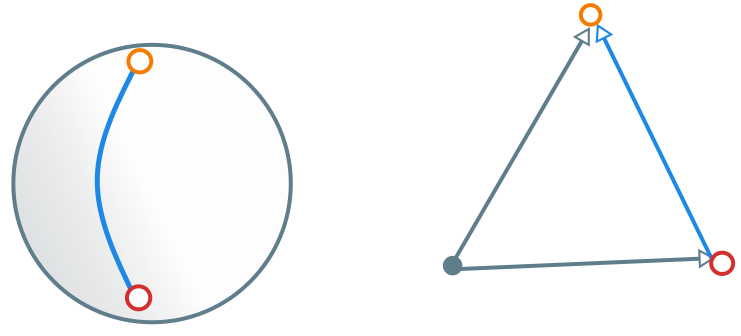
\includegraphics[width=\textwidth]{figures/sphere-shortest-path.png}
\caption{Shortest path on a sphre is a curved path.}
\end{figure}

\section{Generalizing \wtov: Distinction with differences}

In light of the discussion above, we reformulate the informally discussed notions of
points, displacement, and moving along a displacement. We will first describe training, and then
testing where we perform operations such as similarity and analogy.

\subsection{Riemannian Manifolds}
A Riemannian manifold $M$ of dimension $k$ \emph{embedded} in a space of
dimension $n$ is, intuitively, a surface with $k$-degrees of freedom, which has
been embedded in $\R^n$.  For example, a circle has one degree of freedom, the angle $\theta$.
This can be embedded in 2D space $\mathbb R^2$ via the map $\theta \mapsto (\cos \theta, \sin \theta)$.
Similarly, the sphere has two degres of freedom, the azimuthal angle $\theta$ and the angle
at the azimuth $\phi$, and can be mapped into 3D via the map
$(\theta, \phi) \mapsto (\cos \theta \cos \phi, \cos \theta \sin \phi, \sin \theta)$.

% TODO: circle; TODO: sphere.

Here, we assume that the reader is familiar with basic point-set topology \cite{munkres2014topology}.
Formally, the Riemannian manifold of dimension $k$ embedded in a space of dimension $N$
is a subset $M \subseteq \R^N$ such that for each $p \in M$,
there exists an open set $C \subseteq R^k$ (of parameters), and an
an open neighbourhood $O \subseteq \mathbb R^n$ of $p$ (a local parmetrization of $M$ around $p$),
and an onto map $x: C \rightarrow O \cap M$ (of coordinates), such that (1) $x$ is differentiable,
(2) $x$ has a differentiable inverse, and (3) the jacobian of $x$ is one-to-one.
\footnote{We provide the extrinsic definition of a Riemannian manifold as a
subspace of $\mathbb R^n$.  A definition without reference to the embedding
space is an intrinsic definition, which is provided in standard texts, such as
Lee's introduction to smooth manifolds}

Intuitively, a Riemannian manifold allows us to assign co-ordinates at each
local region of the manifold which looks like $\R^N$. For example, the Earth in
total is curved, since it is a sphere. However, around each of us, it is
approximated by a plane, since the Earth appears flat around a small region.
Thus, we can continue to use the differential calculus that we know and love to
compute gradients on a Riemannian manifold, which we will use to perform gradient
descent on curved spaces.

\subsection{Tangent space}
On every manifold, at each point, we have a \emph{tangent space}, which
represents the space of possible directions we can move on the space at that
point. For example, at each point on a circle, we can define a velocity that is
tangential to the circle. See that this space that is tangential is \emph{one dimensional},
even though the circle is itself two-dimensional. The gradient of a function at a point is a
vector which lives in the tangent space a point.

% TODO: add tangent space example.


\subsection{Lie groups}
A lie group is a Riemannian manifold $M$ which is also a group, whose group
structure is compatible with the manifold structure. This means that we have
an associative \emph{group operation} $*: M \times M \rightarrow M$, which comes with an
inverse $(\cdot)^{-1} : M \rightarrow M$, and an identity $e \in M$ such that the group operation $*$
and the inverse $(\cdot)^{-1}$ are continuous with respect to the inherited
subspace topology on $M$.

Intuitively, this gives us the operations (1) $v \cdot w \simeq v + w$ to add
vectors, (2)  $(v)^{-1} \simeq -v$ to invert a vector, and (3) $v \cdot w^{-1} \simeq v - w$
to subtract vectors. This allows us to generalize analogy to curved spaces, by using
lie group operations to perform analogy.

\begin{figure}[htb]
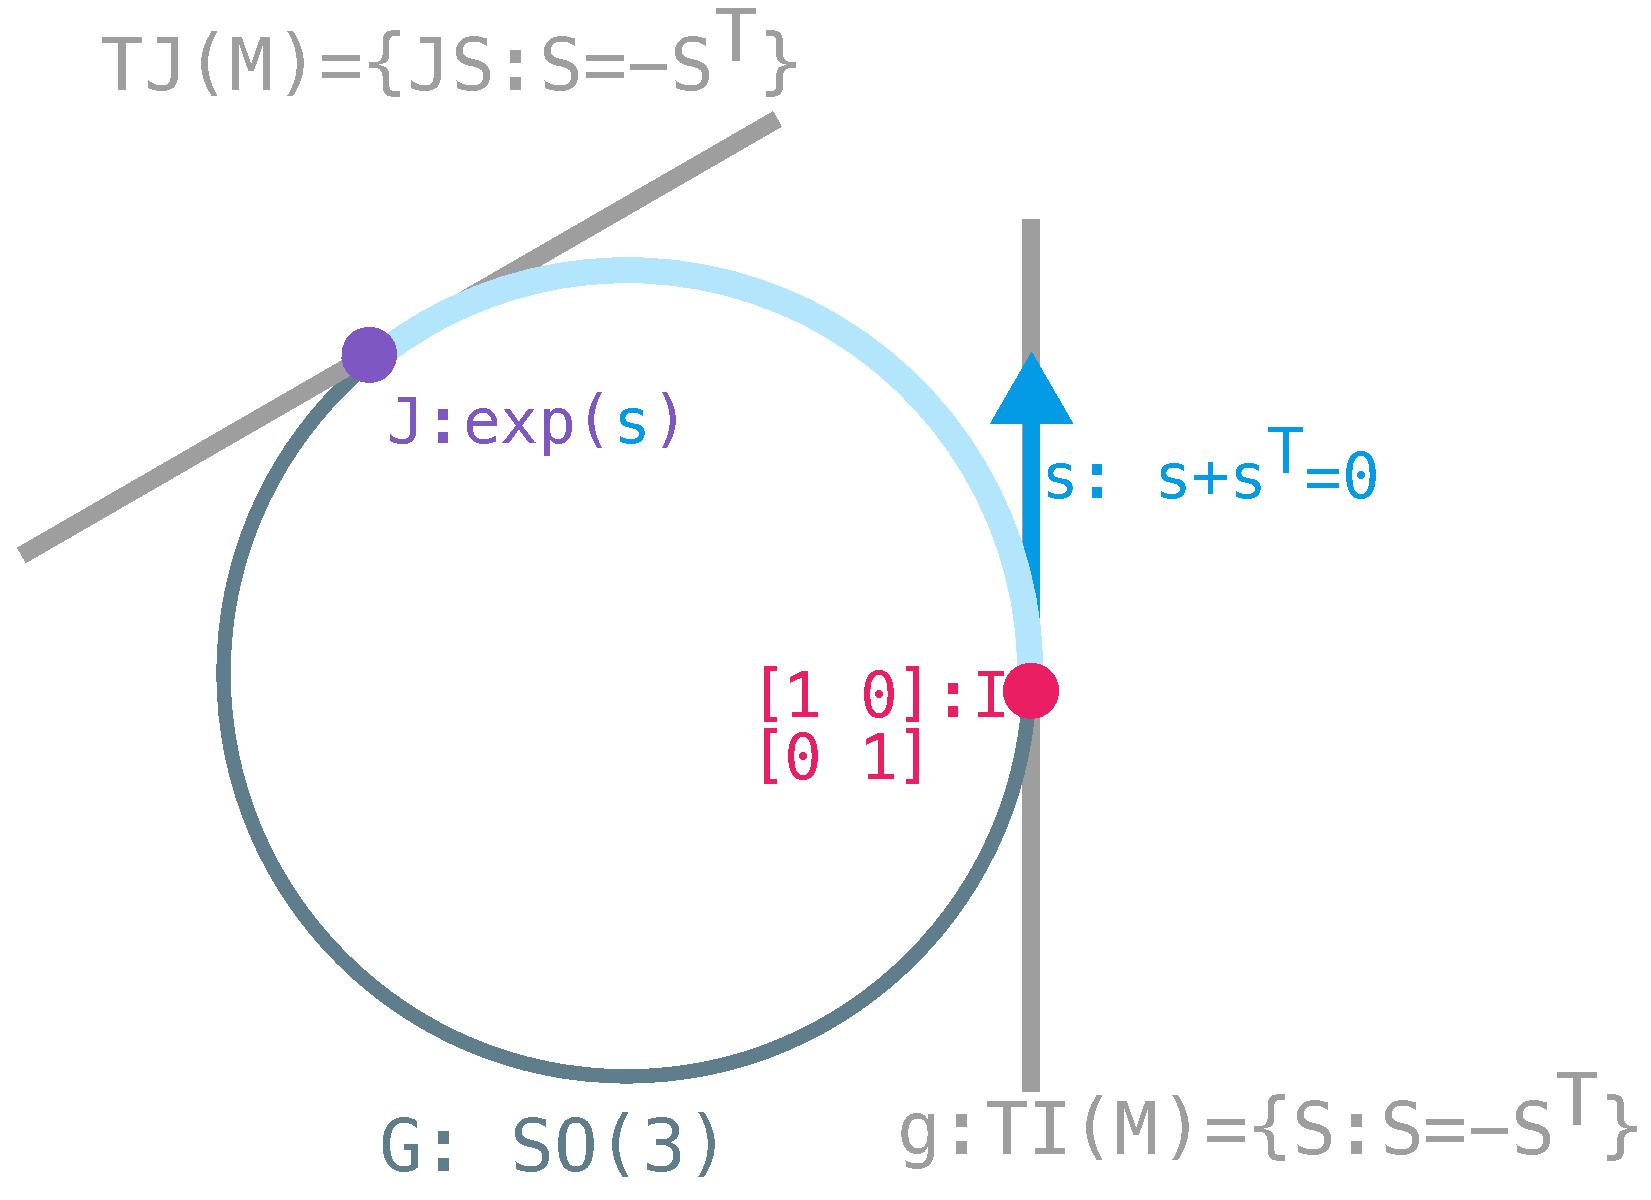
\includegraphics[width=\textwidth]{./lie-group.pdf}
\caption{Lie group}
\end{figure}


\subsection{Lie algebra}
The Lie algebra of a Lie group is the \emph{tangent space} of the Lie group
\emph{at} the identity element. Informally, the idea is that while the Lie group is a
``non-linear'' object, the tangent space represents tangents / ``linearlizations'' of the group.
Moreover, in a group, given a tangent vector at the identity, we can \emph{exponentiate} this
tangent vector to get a Lie group element.

For example, we consider the Lie group of complex numbers of unit norm,
$G \equiv \C^\times = \{ z \in \C : |z| = 1 \}$. The Lie algebra corresponding to $G$, denoted
by $\mathfrak g$ are the real numbers $\mathfrak g = \mathbb R$. We can \emph{exponentiate}
a real number via the map $\exp : \mathfrak g \rightarrow G$, $\exp(r) \equiv e^{i r}$. Similarly,
we have a logarithm map $\log: G \rightarrow \mathfrak g$, which takes any
element $z \in \C^\times$, and produces a real number $\log(z) \equiv arg(z)$.
Notice that the space $\mathfrak g = \mathbb R$ is a real vector space, since it contains an
additive identity $0$, while the space $G = C^\times$ is not a real vector space, since it
is not closed under scaling by reals.

For a more non-trivial example, we consider the space of all rotations in 3D. These are given
by the orthogonal matrices $SO(3) \equiv \{ O : O O ^T = I \}$. We will not derive the Lie algebra
space formally, which can be found in \cite{absil2009optimisation} \footnote{A derivation of the tangent space of $SO(n)$
performed by the author can be found at \url{https://math.stackexchange.com/questions/3389983/explicit-description-of-tangent-spaces-of-on}}.
Informally, the idea is that the Lie algebra represents a logarithmization of the tangent space. Thus,
we must compute $\log(SO(3)) = \{ \log(O): \log(O O^T) = \log(I) \}$. This leads to the calculation:

\begin{align*}
&\log(SO(3)) = \{ \log(O): \log(O O^T) = \log(I) \} \\
&\log(SO(3)) = \{ \log(O): \log(O) + \log(O^T) = \log(I) \} \\
&\log(SO(3)) = \{ \log(O): \log(O) + \log(O)^T = \log(I) \} \\
&\log(SO(3)) = \{ \log(O): \log(O) + \log(O)^T = 0 \} \\
&\skewsym = \{ Z: Z + Z^T = 0 \} \\
\end{align*}

Thus, the tangent space of $SO(3)$ is the space $\skewsym$ of skew-symmetric matrices. Notice that skew symmetric
matrices form a vector space, since the sum of two skew symmetric matrices is skew-symmetric, and skew-symmetric
matrices are closed under scaling by the real numbers. On the other hand, $SO(3)$ is not a vector space; For example,
the element $I \in SO(3)$ as $I I^T = I$. On the other hand, consider $J \equiv 2I$. We have
$J J^T = 4I \neq I$. Thus $SO(3)$ is not closed under scaling by reals, and is thus not a vector space. Hence,
we see that even in this case, the Lie group is not a vector space, while the Lie algebra is a vector space.
Philosophically, skew-symmetric matrcies correspond to angular momenta, which are indeed the ``velocities''
of a rotation.

\todo{For each section, also add linguistic corollaries. This will make it a bit
  easier to digest the transition from dense math topic to dense math topic}

\subsubsection{Setting} We will now be imagining our words as \emph{elements of a lie group}. Recall that this means that
they are points in some \emph{subspace} of $\mathbb R^n$, where this subspace can be curved in shape.
Also, the elements are equipped with the notion of a logarithm; That is, they come equipped with a
function $\log : G \rightarrow \mathfrak g$, and $\exp: \mathfrak g \rightarrow G$,
where $\log$ maps from the lie group (a group) to its lie algebra (a vector space),
and vice versa for the $\exp$ map.


\subsubsection{Dot Product}  To compute the dot product between two elements $g, h \in G$, we first logarithmize
them, and then take the dot product of their logarithms, which lives in the Lie algebra.
Hence, we define the dot product on the Lie group $\langle \cdot , \cdot \rangle$ as
$\langle g, h \rangle \equiv \log(g) \cdot \log(h)$.


\subsubsection{Gradients} Next, to perform gradient descent, we need
a notion of a \emph{gradient} to decide in which direction to move, and a way to perform a gradient update.
How one performs the gradient update is explained in detail in the \label{section:optim-on-riem}. Intuitively,
since all our manifolds are subspaces of $\mathbb R^n$, we first compute the gradient vector, then travel
along the gradient vector (which will take us out of the manifold), and finally ``retract back'' into the
manifold, which gives us a gradient step, starting from a point in the manifold, ending at a point in the manifold.

\begin{figure}[htb]
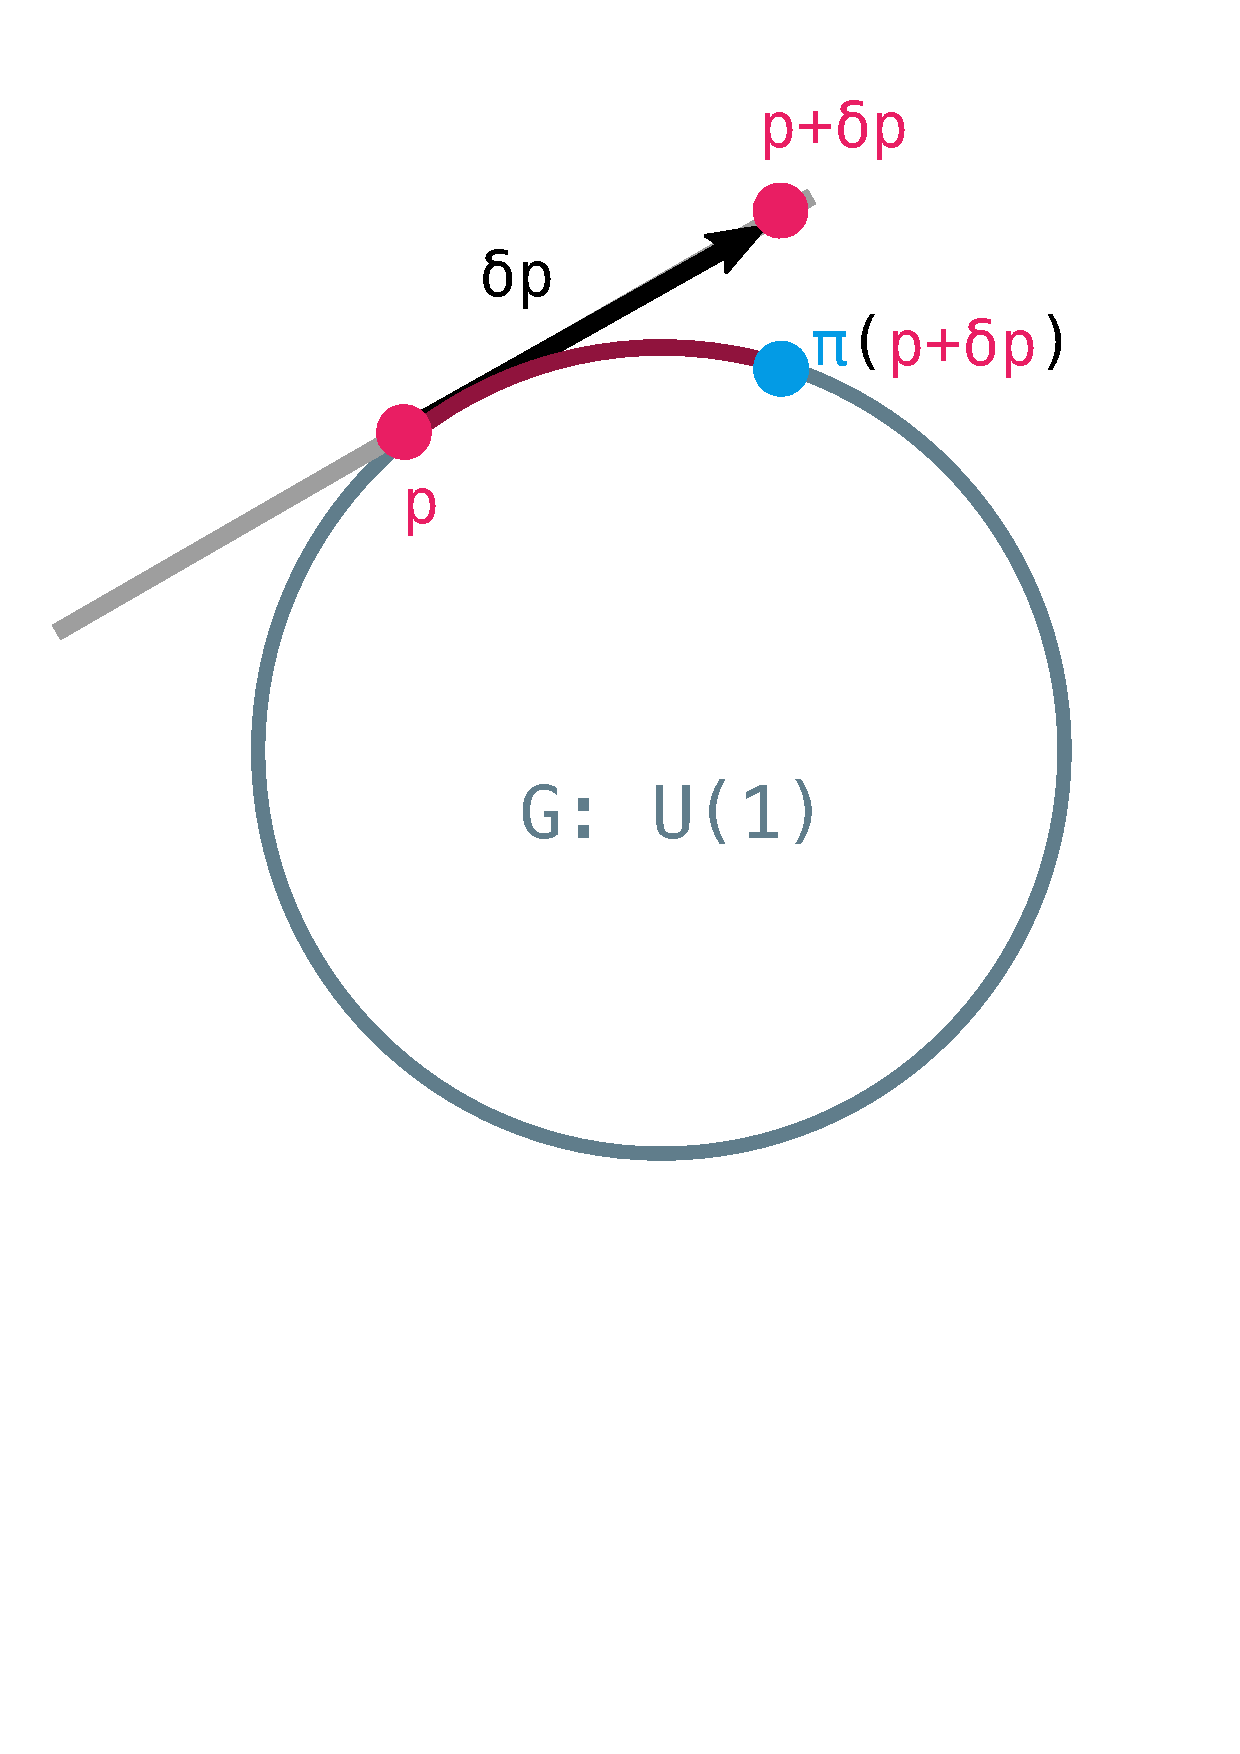
\includegraphics[width=0.5\textwidth]{./gradient-manifold.pdf}
\caption{gradient descent on a manifold.}
\end{figure}

\todo{Differentiate sections into math basics, training, and evaluation.}

\subsubsection{Similarity} We compute similarity between two words by computing the dot product between
the vectors which represent the words.

\todo{Pls detail xD}

\subsubsection{Displacement} To compute the displacement from one word $v$ to another word $w$, we compute the element $d \equiv (v \cdot w^{-1})$.
See that $d \cdot w = (v \cdot w^{-1}) \cdot w = v$. That is, moving along $d$ from $w$ produces a $v$.

\todo{revisit minorly the difference v. displacement argument}

\subsubsection{Moving along displacement} To perform a analogy given a displacement $d$ and a basepoint $p$, we compute $d \cdot p$.

\todo{elaboration}

\section{Optimisation on Riemannian Manifolds}
\label{section:optim-on-riem}.

\todo{introduce the need: ML algorithms and all that}

We now consider manifold optimisation techniques on embedded riemannian manfiolds $M$,
equipped with the metric $g: (p: M) \rightarrow T_p M  \times T_p M \rightarrow \mathbb R$.
The metric at a point $g(p)$ provides an inner product structure on the point $T_pM$
for a $p \in M$.

where we are optimising a cost function $c: M \rightarrow \mathbb R$.
We presume that we have a diffeomorphism $E: M \rightarrow \mathbb R^n$ (Embedding) which
preserves the metric structure. We will elucidate this notion of preserving
the metric structure once we formally define the mapping between tangent spaces.
This allows us to treat $M$ as a subspace of $\mathbb R^n$.

For any object $X$
defined with respect to the manifold, we define a new object $\overline X$, which
is the embedded version of $X$ in $\mathbb R^n$.

We define $\overline M \subset \mathbb R^n; \overline M \equiv image(E)$.
We define $\overline c: \overline M \subseteq \mathbb R^n \rightarrow \mathbb R; \overline c \equiv c \circ E^{-1}$

We then needh two operators, that allows us to project onto the tangent space
and the normal space. The tangent space at a point $x_0 \in M$, $\overline{T_{x_0} M} \equiv span(\partial_i E |_{E(x_0)})$.
We get an induced mapping of tangent spaces $dE: T_{x_0} M$ and $T_{x_0} \overline M$.

we consider the gradient
$\overline \grad c : (p: \overline M) \rightarrow \overline{T_p M}; \overline \grad c \equiv dE \overline dc$

The normal space,
$\overline{N_{x_0} M}$ is the orthogonal complement of the tangent space, defined
as $\overline{N_{x_0} M} \equiv \left\{ v \in \mathbb R^n \mid \langle v | \overline{T_{x_0} M} \rangle = 0 \right\}$.
It is often very easy to derive the projection onto the normal space, from
whose orthogonal complement we derive the projection of the tangent space.

The final piece that we require is a retraction $R: \mathbb R^n \rightarrow \overline M \subseteq \mathbb R^n$. This allows
us to project elements of the ambient space that are not on the manifold. The
retraction must obey the property $R(p \in \overline M) = p$.
% (TODO: is this correct? Do we need $R(\overline M) = \overline M$ or is this pointwise?)
% (what are the other conditions on the retraction? smoothness?)

Given all of this machinery, the algorithm is indeed quite simple.

\begin{itemize}
	\item $x \in \overline M \subseteq \mathbb R^n$ is the current point on the manifold as an element of $\mathbb R^n$
	\item Compute $g = \grad c(x) \in T_x \mathbb R^n$ is the gradient with respect to $\mathbb R^n$.
	\item $\overline g = P_{T_x} g \in T_x M$ is the projection of the gradient with respect to $\mathbb R^n$ onto the
	tangent space of the manifold.
	\item $x_{mid}\in \mathbb R^n \equiv x + \eta \overline g$, a motion along the tangent vector, giving a point in
	$\mathbb R^n$.
	\item $\overline x_{next}: \overline M \equiv R(x_{mid})$, the retraction of the motion along the tangent vector,
	giving a point on the manifold $\overline M$.
\end{itemize}


We point out that this algorithm, when specialized to $\mathbb R^n$ as a Lie
group recovers the fuzzy set representation, where we perform similarity and
analogy on the \emph{logarithmized inputs}, which we interpreted as treating
\texttt{word2vec} vectors as fuzzy sets. We leave the experimentation on more
exotic manifolds as open for future work.

%--------------------------------------------------------
%%% Optional appendix
%\appendix
%\chapter{}
%\label{}

\chapter{Conclusion and Future Work}

\epigraph{A good proof is one that makes us wiser.}{Yuri Manin}

In this thesis, we focus on \emph{empirical study} to provide
\emph{mathematical} formalisms for word embeddings. Towards this goal, we
provide two directions of research: One based on the linguistic theory of
Montague semantics, which we link to the formal theory of abstract
interpretation, from which we produce fuzzy set representations. These fuzzy
embeddings are extracted from standard word embeddings, and provide access to
set theoretic and probabilistic operations on word embeddings. This exhibits
our conjecture that word embeddings are in fact capturing montagueian based
semantics. The second prong of our research is purely mathematical, where we
analyze the conflation of various ideas in classical word embeddings, and
dis-entangle these ideas to provide a framework for generating word embeddings
over Lie groups.  We see that our generalization provides a cleaner framework
to \emph{think} about word embeddings, where we provide separate mathematical
objects that captures notions of similarity, analogy, meaning distance, and
meaning interpolation.  For the future, we envision lines of research which
exploits other geometric structures posessed by the manifold, including notions
of \emph{parallel transport}, which provide a notion of interpolation of word
meaning. Furthermore, we wish to adapt results from PAC learning --- in
particular the contrastive losses \cite{arora2019theoretical} to our
generalized setting of Lie groups.  In closing, I hope this thesis has given
you, the reader, a glimpse into pretty mathematical abstractions, reified by
the humble \texttt{word2vec}.


%--------------------------------------------------------
% Recommended 'Related Publication'
\chapter*{Related Publications}
\label{ch:relatedPubs}
% \input{relatedPapers.tex}


Word Embeddings as Tuples of Feature Probabilities: \textbf{Siddharth Bhat},
Alok Debnath, Souvik Banerjee, Manish Shrivastava - Proceedings of the 5th
Workshop on Representation Learning for NLP, 2020


%--------------------------------------------------------
\nocite{*}
\bibliographystyle{latex8}
%\bibliography{References,Introduction/References} % To include one or more reference.bib files
% \bibliography{references}
\bibliography{references}

\end{document}
